\chapter{Foundations of packet simulation}
\section{The symmetry-collapse question}
\label{s:ch:question}
\index{symmetry collapse}

\subsection{The computational mismatch}
An $n$-qubit pure state has $2^n$ complex amplitudes in the computational basis. That description is universal but frequently redundant. A number-preserving circuit started with two excitations never visits basis strings of weight zero, one, three, or more. A permutation-symmetric circuit started in a symmetric state never distinguishes two strings that differ only by a relabeling of qubits. A quantum walk on a highly symmetric graph may evolve entirely in the span of a polynomial number of orbit states. In each case the full Hilbert space is a valid container but not the intrinsic state space of the computation.

The question is therefore not whether a quantum circuit acts on an exponential ambient space. It is whether the reachable part of that space, together with the gate action and measurement, has a polynomial classical representation.

\begin{definition}[Exact symmetry collapse]
A uniform quantum circuit family exhibits an exact symmetry collapse when its acceptance probability can be computed by an exact classical simulation on an invariant representation whose description and update costs are polynomial in the input length.
\end{definition}

\begin{definition}[Approximate symmetry collapse]
A uniform circuit family exhibits an approximate symmetry collapse to error $\varepsilon(n)$ when a polynomial-size classical representation reproduces its acceptance probability to additive error $\varepsilon(n)$, with the error below the promise gap required by the decision problem.
\end{definition}

\subsection{Four conclusions that must not be conflated}
The phrase ``symmetry reduction'' is used for several logically different achievements.

\begin{enumerate}
\item \textbf{Structural reduction.} A projector, quotient, or representation-theoretic coordinate change removes redundant coordinates.
\item \textbf{Practical acceleration.} A concrete implementation uses less time or memory on tested instances.
\item \textbf{Polynomial classical simulation.} A uniform family admits a deterministic polynomial-time classical algorithm.
\item \textbf{Universal complexity collapse.} Every polynomial-size quantum circuit admits such a representation.
\end{enumerate}

The first three occur in this monograph for declared subclasses. The fourth would imply $BQP\subseteq P$ and is not established. A benchmark can support the second conclusion without proving the third. A small invariant label set can support the first conclusion while leaving exponentially large internal blocks and therefore failing to prove the third.

\subsection{The four audit quantities}
For a proposed reduction, define the schematic complexity record
\[
\mathfrak C_n=
\bigl(
N_{\mathrm{packets}},
D_{\mathrm{internal}},
S_{\mathrm{transfer}},
L_{\mathrm{leakage}}
\bigr).
\]
Here:

\begin{itemize}
\item $N_{\mathrm{packets}}$ is the number of reachable symmetry labels.
\item $D_{\mathrm{internal}}$ is the packet dimension or the size of a compressed internal representation.
\item $S_{\mathrm{transfer}}$ records the sparsity and cost of gate-induced transitions.
\item $L_{\mathrm{leakage}}$ measures departure from the proposed representation.
\end{itemize}

A complete claim must also state the cost of discovering this structure from the input. A decomposition that is small but exponentially hard to find does not yield a polynomial algorithm.

\begin{figure}[H]
\centering
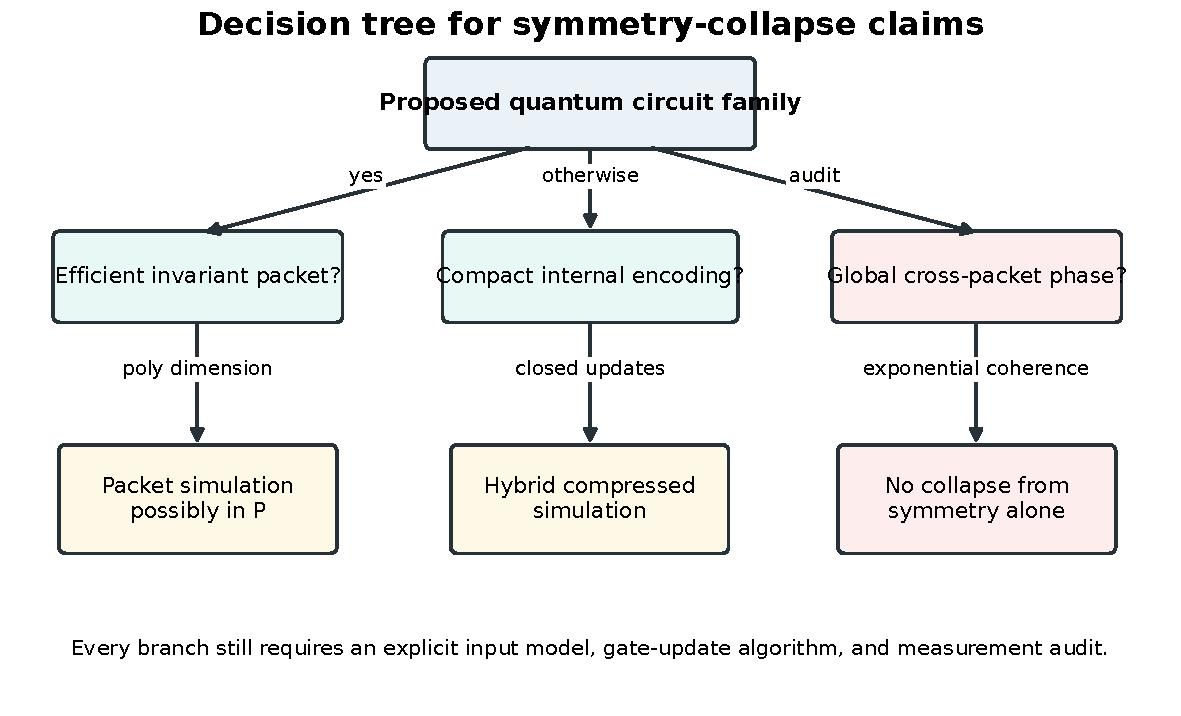
\includegraphics[width=.91\textwidth]{assets/s_collapse_decision_tree.pdf}
\caption{A disciplined decision tree for proposed symmetry-collapse claims.}
\end{figure}

\subsection{Why symmetry is only the beginning}
Suppose a group $G$ acts on the Hilbert space and the circuit commutes with this action. Representation theory decomposes the space into isotypic pieces. This gives a canonical block structure, but three questions remain.

First, how many pieces are reachable from the input? Second, how large is each piece or how compactly can its states be encoded? Third, can each gate and measurement be applied in those coordinates without reconstructing the full state? The monograph repeatedly returns to this three-stage distinction:
\[
\text{symmetry label}
\longrightarrow
\text{reachable representation}
\longrightarrow
\text{efficient classical algorithm}.
\]

\begin{principle}[No free collapse]
Block diagonality is a structural statement. Polynomial-time classical simulation requires an efficient basis or encoding, efficient updates, and efficient output evaluation in addition to the block decomposition.
\end{principle}

\section{Projectors and quantum packets}
\label{s:ch:projectors}
\index{projector}
\index{packet decomposition}

\subsection{Orthogonal packet decompositions}
Let $\Hh$ be a finite-dimensional Hilbert space and let $\{P_\alpha\}_{\alpha\in A}$ be orthogonal projectors satisfying
\[
P_\alpha P_\beta=\delta_{\alpha\beta}P_\alpha,
\qquad
\sum_{\alpha\in A}P_\alpha=I.
\]
Every state and operator decompose as
\[
\ket\psi=\sum_\alpha P_\alpha\ket\psi,
\qquad
X=\sum_{\alpha,\beta}P_\alpha X P_\beta.
\]
The diagonal blocks act within packets. The off-diagonal blocks transfer amplitude or coherence between packets.

Define the packet-transfer graph of an operator $X$ by placing an edge $\beta\to\alpha$ whenever
\[
P_\alpha X P_\beta\neq0.
\]
An exactly symmetry-preserving operator has only diagonal edges. A sparse transfer graph may still permit efficient simulation if the active packets and internal states remain compact.

\subsection{Conserved observables}
Let
\[
Q=\sum_k q_kP_k
\]
be a self-adjoint observable with spectral projectors $P_k$.

\begin{theorem}[Invariant quantum packets]
\label{s:thm:invariant-packets}
If a unitary $U$ satisfies $[U,Q]=0$, then
\[
P_iUP_j=0\qquad(i\neq j),
\]
and
\[
U=\bigoplus_i U_i,
\qquad
U_i=P_iUP_i\big|_{P_i\Hh}.
\]
If $P_k\ket\psi=\ket\psi$, then $P_kU\ket\psi=U\ket\psi$.
\end{theorem}

\begin{proof}
Since $U$ commutes with $Q$, it commutes with every spectral projector obtained from the functional calculus of $Q$. Thus
\[
P_iUP_j=UP_iP_j=0
\]
for $i\neq j$. Summing the diagonal blocks gives the direct-sum form. The final statement follows from
\[
P_kU\ket\psi=UP_k\ket\psi=U\ket\psi.
\]
\end{proof}

\subsection{Residue and character packets}
Suppose $Q$ has integer spectrum. For a modulus $M$, define
\[
B_r^{(M)}=
\sum_{k\equiv r\pmod M}P_k.
\]
Let
\[
V_M=\exp\left(\frac{2\pi i}{M}Q\right),
\qquad
\omega_M=e^{2\pi i/M}.
\]
Then
\begin{equation}
B_r^{(M)}
=
\frac1M\sum_{\ell=0}^{M-1}
\omega_M^{-r\ell}V_M^\ell.
\label{s:eq:residue-projector}
\end{equation}
On a $Q$-eigenvector, the right side is the roots-of-unity filter. The same finite-character formula selects residue classes in signal polyphase analysis and charge sectors in quantum theory.

\subsection{Finite-group projectors}
Let a finite group $G$ act unitarily by $U_g$. For an irreducible character $\chi$ of degree $d_\chi$, the central isotypic projector is
\begin{equation}
P_\chi
=
\frac{d_\chi}{|G|}
\sum_{g\in G}
\overline{\chi(g)}U_g.
\label{s:eq:character-projector}
\end{equation}
Character orthogonality gives
\[
P_\chi P_\psi=\delta_{\chi\psi}P_\chi,
\qquad
\sum_\chi P_\chi=I
\]
on the represented space. If an operator $A$ commutes with every $U_g$, then
\[
P_\chi A P_\psi=0
\qquad(\chi\neq\psi).
\]

This framework includes momentum, parity, total spin, point-group symmetry, permutation symmetry, and stabilizer syndrome labels. The isotypic projector identifies a symmetry type. It does not necessarily resolve the multiplicity space within that type.

\subsection{Nested refinements}
If one conserved label is too coarse, intersect commuting projector families. For mutually commuting observables $Q_1,\ldots,Q_s$, a joint packet has the form
\[
P_{\bm\alpha}
=
P^{(1)}_{\alpha_1}\cdots P^{(s)}_{\alpha_s}.
\]
The dimension can decrease dramatically, but each extra label must be efficiently computable and preserved. A refinement that requires exponential preprocessing merely relocates the complexity.

\begin{remark}
A packet decomposition is basis independent as an orthogonal direct sum, although a practical simulator must choose a concrete basis or compressed coordinate system within each active packet.
\end{remark}

\section{Uniform circuits and the classical cost model}
\label{s:ch:complexity-model}
\index{uniform circuit}
\index{classical simulation}

\subsection{Circuit families}
A quantum decision procedure is a polynomial-time uniform family of circuits $\{C_x\}$, where the input string $x$ determines a circuit on $n=n(|x|)$ qubits with at most $\poly(|x|)$ gates. Let
\[
C_x=G_m\cdots G_1.
\]
A classical simulation theorem must describe an algorithm receiving the same succinct description of $x$ and the circuit. It is not enough to assume that an exponentially large matrix or a complete orbit list has already been supplied.

\subsection{The packet access model}
For each input length, suppose there is a packet projector $P_n$ and a basis
\[
\B_n=
\{\ket{b_1},\ldots,\ket{b_{D_n}}\}
\]
of $P_n\Hh_n$. The simulation interface has four routines.

\begin{enumerate}
\item \textbf{Discovery and indexing.} Produce or index $\B_n$ in polynomial time.
\item \textbf{Initialization.} Express the initial state in this basis.
\item \textbf{Gate update.} Apply each restricted gate $P_nG_jP_n$ to the packet coordinates in polynomial time.
\item \textbf{Measurement.} Compute the final acceptance probability to the needed precision.
\end{enumerate}

The basis need not be listed explicitly if there is a compact data structure supporting these operations. Stabilizer tableaux and covariance matrices are examples of representations that encode exponentially many computational-basis amplitudes without storing them individually.

\subsection{Precision and promise gaps}
A BQP decision problem has an inverse-constant promise gap after standard amplification. A deterministic classical simulator need only estimate the acceptance probability to an additive error smaller than this gap. If the gate entries are algebraic or otherwise polynomial-time computable, ordinary numerical analysis gives polynomial bit complexity for polynomially many updates, provided condition numbers and error amplification are controlled.

\subsection{State-vector cost inside a packet}
If the simulator stores $D$ amplitudes and a local gate can be applied in $O(nD)$ arithmetic operations, a depth-$d$ packet simulation has schematic cost
\[
C_{\mathrm{packet}}=O(dnD)+C_{\mathrm{compile}}.
\]
The corresponding full state-vector path is
\[
C_{\mathrm{full}}=O(dn2^n).
\]
These formulas are intentionally schematic. Cache behavior, indexing, vectorization, and basis compilation determine actual runtime. The asymptotic distinction is exact when $D$ is polynomial and $2^n$ is exponential.

\subsection{Reuse and amortization}
Packet compilation can be expensive. Repeated parameter sweeps, time stepping, variational optimization, and repeated likelihood evaluation benefit from cached basis maps and gate plans. A one-shot simulation can be slower even when each subsequent packet update is much cheaper. The benchmark chapter preserves both one-shot and repeated-application measurements for this reason.

\begin{scopebox}
A polynomial-dimensional invariant sector does not guarantee a practical speedup at small $n$. It guarantees that the state-vector representation within that sector has polynomial asymptotic size under the stated access assumptions.
\end{scopebox}

\section{Exact packet simulation and polynomial collapse}
\label{s:ch:exact-simulation}

\subsection{Gatewise invariance}
Let $P$ be an orthogonal projector and suppose the initial state obeys $P\ket{\psi_0}=\ket{\psi_0}$. If every gate satisfies
\begin{equation}
G_jP=PG_jP,
\label{s:eq:gatewise-invariance}
\end{equation}
then $G_j$ maps $P\Hh$ into itself. For a general linear map, this equation asserts only invariance of the selected subspace. For the finite-dimensional unitary gates considered here, invariance also implies invariance of the orthogonal complement, so it is equivalent to commutation with $P$.

\begin{theorem}[Invariant-basis simulation]
\label{s:thm:invariant-basis}
Let $U=G_m\cdots G_1$ and assume \cref{s:eq:gatewise-invariance} for every gate. If $P\ket{\psi_0}=\ket{\psi_0}$, then
\[
U\ket{\psi_0}
=
(PG_mP)\cdots(PG_1P)\ket{\psi_0}.
\]
In any basis of $P\Hh$, the restricted circuit gives exactly the same amplitudes after embedding.
\end{theorem}

\begin{proof}
Inductively, if $P\ket{\psi_{j-1}}=\ket{\psi_{j-1}}$, then
\[
G_j\ket{\psi_{j-1}}
=
G_jP\ket{\psi_{j-1}}
=
PG_jP\ket{\psi_{j-1}},
\]
so the next state remains in $P\Hh$. Iterating proves the identity.
\end{proof}

\subsection{Polynomial packet-simulation theorem}
\begin{theorem}[Polynomial packet-simulation theorem]
\label{s:thm:poly-packet}
Let $\{C_x\}$ be a polynomial-time uniform family of quantum circuits. Suppose there is an efficiently computable packet representation such that:

\begin{enumerate}
\item the initial state lies in the represented packet and its coordinates are computable in polynomial time;
\item every gate preserves the representation;
\item the representation size is at most $\poly(|x|)$;
\item each gate update is computable to polynomial precision in polynomial time;
\item the final acceptance probability is computable from the representation in polynomial time.
\end{enumerate}

Then the language decided by the circuit family belongs to $P$.
\end{theorem}

\begin{proof}
The simulator stores a polynomial-size classical description of the evolving state. It performs polynomially many polynomial-time gate updates and evaluates the final measurement to inverse-polynomial precision. Choosing an error smaller than the amplified promise gap yields a deterministic polynomial-time decision algorithm.
\end{proof}

\begin{provedbox}
The theorem is a genuine quantum-to-classical complexity collapse for the declared subclass. It does not assume that a full $2^n$ state vector is ever constructed.
\end{provedbox}

\subsection{Dimension-only corollary}
A convenient special case uses an explicit basis of a packet of dimension $D_n$.

\begin{corollary}[Polynomial-dimensional invariant packet]
If $D_n\le\poly(n)$, the packet basis is efficiently indexed, every gate has a polynomial-time sparse or structured action in that basis, and the measurement is efficiently evaluable, then the circuit family is classically polynomial-time simulable.
\end{corollary}

\subsection{A broader compressed representation}
The state description need not be a vector of packet amplitudes. Let $\mathcal R_n$ be a polynomial-size classical representation class with an embedding into the packet Hilbert space. If initialization, gate updates, and measurement stay within $\mathcal R_n$ and are efficient, the same proof applies. This observation will later combine packet labels with stabilizer, Gaussian, or tensor-network coordinates.

\begin{figure}[H]
\centering
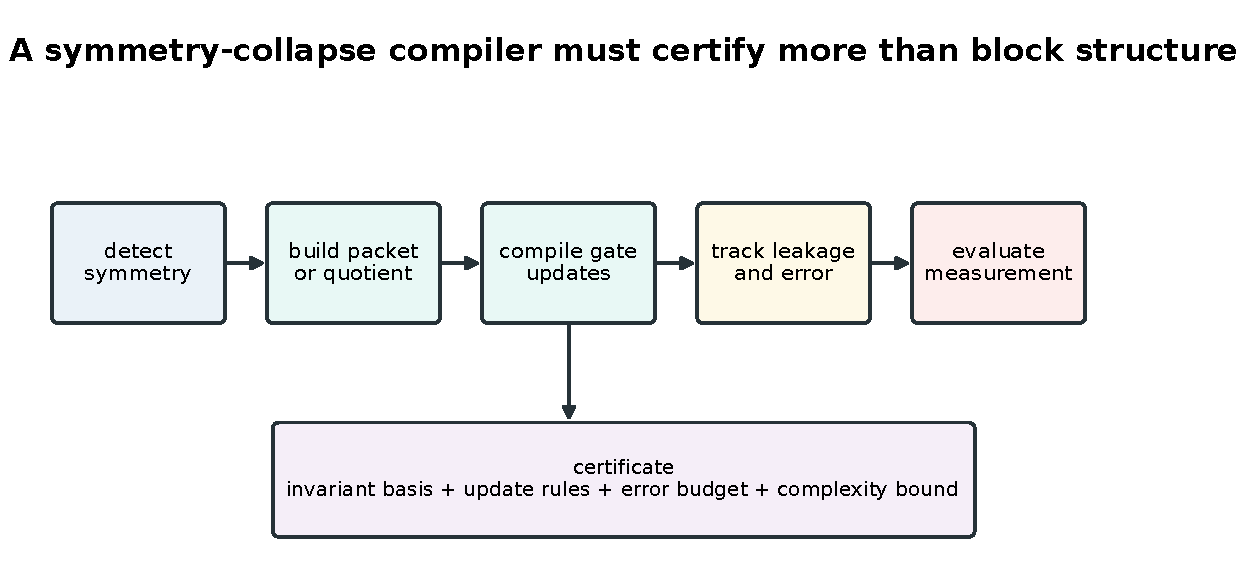
\includegraphics[width=.92\textwidth]{assets/s_compiler_pipeline.pdf}
\caption{A complete collapse certificate includes discovery, update, leakage, measurement, and complexity information.}
\end{figure}

\section{Approximate symmetry and leakage certificates}
\label{s:ch:approximate-symmetry}
\index{leakage}

\subsection{Hamiltonian leakage}
Exact conservation is not the only useful regime. Let $P$ be an orthogonal projector and let
\[
U(t)=e^{-itH}
\]
for a bounded self-adjoint Hamiltonian $H$. The leakage operator from the packet is
\[
L_P(t)=(I-P)e^{-itH}P.
\]

\begin{theorem}[Commutator leakage bound]
\label{s:thm:commutator-leakage}
For every real $t$,
\[
\|(I-P)e^{-itH}P\|
\le
|t|\,\|[H,P]\|.
\]
\end{theorem}

\begin{proof}
Define
\[
F(s)=e^{-i(t-s)H}Pe^{-isH}P.
\]
Then $F(0)=e^{-itH}P$ and $F(t)=Pe^{-itH}P$. Differentiation gives
\[
F'(s)=ie^{-i(t-s)H}[H,P]e^{-isH}P.
\]
Therefore
\[
(I-P)e^{-itH}P
=-(I-P)\int_0^tF'(s)\,ds.
\]
The unitary factors and projectors have norm at most one, so the integral is bounded by $|t|\|[H,P]\|$.
\end{proof}

\subsection{Circuit leakage}
For a gate $G_j$, define
\[
\delta_j=\|(I-P)G_jP\|.
\]
Let $V_j=PG_jP$. A telescoping expansion gives
\[
G_m\cdots G_1P-V_m\cdots V_1P
=
\sum_{k=1}^m
G_m\cdots G_{k+1}(G_k-V_k)V_{k-1}\cdots V_1P.
\]
Taking norms yields the following.

\begin{proposition}[Sum-of-leakages bound]
\label{s:prop:sum-leakage}
For an initial state in $P\Hh$,
\[
\|G_m\cdots G_1\ket{\psi_0}
-
V_m\cdots V_1\ket{\psi_0}\|
\le
\sum_{j=1}^m\delta_j.
\]
\end{proposition}

This is conservative because leakage contributions may interfere destructively. Its value is that it is composable and can be checked gate by gate.

\subsection{Decision-problem consequence}
If the packet representation is polynomial, the restricted updates are efficient, and
\[
\sum_j\delta_j\le\frac1{\poly(n)},
\]
then the approximate packet simulator reproduces the final acceptance probability to inverse-polynomial accuracy. After ordinary promise-gap amplification, this suffices for a deterministic polynomial-time decision algorithm.

\subsection{Adaptive packet enlargement}
A practical simulator need not fix one packet forever. It can maintain an active set $A_t$ of packets, estimate transfers $P_\alpha G_tP_\beta$, and add a packet when its predicted mass exceeds a tolerance. The proof obligation becomes a global accounting identity:
\[
\text{total error}
\le
\text{discarded transfer}
+
\text{numerical error}
+
\text{measurement approximation}.
\]
The key research problem is to retain polynomial active size while certifying the tail.

\begin{figure}[H]
\centering
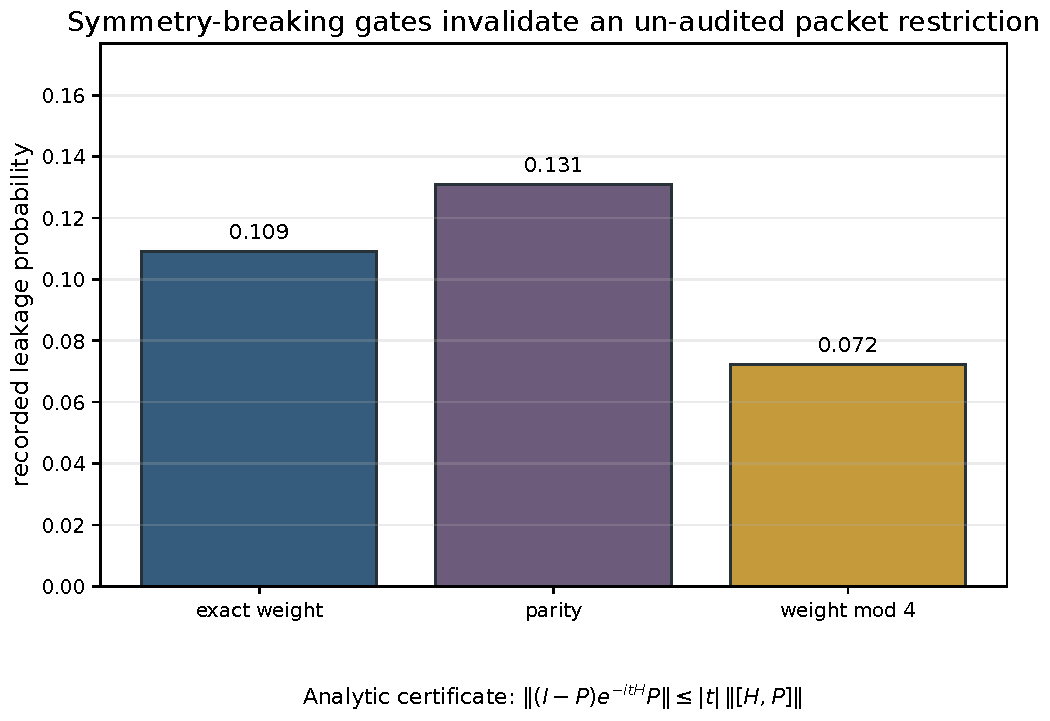
\includegraphics[width=.76\textwidth]{assets/s_leakage_bound.pdf}
\caption{Recorded leakage examples and the analytic commutator certificate.}
\end{figure}

\section{Moving packets, dynamic frames, and sparse transfer graphs}
\label{s:ch:dynamic-frames}
\index{moving packet}
\index{time-dependent projector}
\index{packet transfer graph}

\subsection{Why one fixed projector is not the end of the theory}
The exact packet theorem in \cref{s:ch:exact-simulation} follows a state inside one fixed subspace. That is sufficient for a conserved charge, but it is not necessary for classical collapse. A circuit may move through a sequence of small subspaces, or it may preserve a small packet only after a time-dependent change of coordinates. The correct object is therefore a \emph{packet schedule}, not necessarily one static projector.

\begin{definition}[Packet schedule]
For a circuit
\[
U=G_m\cdots G_1
\]
on a Hilbert space $\Hh$, a packet schedule is a sequence of orthogonal projectors
\[
P_0,P_1,\ldots,P_m.
\]
It is exact when
\begin{equation}
G_tP_{t-1}=P_tG_tP_{t-1}
\qquad(1\le t\le m).
\label{s:eq:dynamic-packet-condition}
\end{equation}
\end{definition}

The condition says that gate $G_t$ maps the currently active packet into the next active packet. The dimensions may vary with time.

\subsection{Exact dynamic-packet simulation}
Choose isometries
\[
B_t:\C^{D_t}\longrightarrow\Hh,
\qquad
B_tB_t^*=P_t,
\qquad
B_t^*B_t=I_{D_t},
\]
where $D_t=\rank P_t$. Define the rectangular coordinate update
\begin{equation}
M_t=B_t^*G_tB_{t-1}.
\label{s:eq:dynamic-coordinate-update}
\end{equation}

\begin{theorem}[Exact dynamic-packet theorem]
\label{s:thm:dynamic-packet}
Suppose $P_0\ket{\psi_0}=\ket{\psi_0}$ and \cref{s:eq:dynamic-packet-condition} holds for every gate. Put
\[
z_0=B_0^*\ket{\psi_0},
\qquad
z_t=M_tz_{t-1}.
\]
Then
\[
G_t\cdots G_1\ket{\psi_0}=B_tz_t
\]
for every $t$.
\end{theorem}

\begin{proof}
The claim is true at $t=0$. If the state after $t-1$ gates is $B_{t-1}z_{t-1}$, then
\[
G_tB_{t-1}z_{t-1}
=P_tG_tP_{t-1}B_{t-1}z_{t-1}
=B_tB_t^*G_tB_{t-1}z_{t-1}
=B_tM_tz_{t-1}.
\]
This is $B_tz_t$.
\end{proof}

\begin{theorem}[Polynomial moving-packet collapse]
\label{s:thm:moving-packet-collapse}
Let $\{C_x\}$ be a polynomial-time uniform circuit family. Suppose an exact packet schedule can be produced from $x$ in polynomial time such that:
\begin{enumerate}
\item $\max_tD_t\le\poly(|x|)$;
\item the coordinate description of the initial state is computable in polynomial time;
\item each rectangular update $M_t$ can be applied to polynomial precision in polynomial time;
\item the final acceptance probability is computable from $z_m$ in polynomial time.
\end{enumerate}
Then the language decided by the circuit family belongs to $P$.
\end{theorem}

\begin{proof}
The simulator stores at most polynomially many coordinates at every step and applies polynomially many polynomial-time updates. \Cref{s:thm:dynamic-packet} proves exactness before numerical rounding. Polynomial precision below the amplified promise gap gives a deterministic polynomial-time decision procedure.
\end{proof}

\begin{derivedbox}
A circuit does not need one globally conserved sector. It is enough that the state follow an efficiently discoverable path through polynomial-dimensional sectors.
\end{derivedbox}

\subsection{Moving frames and hidden symmetry}
The packet schedule has a useful coordinate form. Let $P$ be one fixed projector and let $W_t$ be unitaries with
\[
P_t=W_tPW_t^*.
\]
In the moving frame, the transformed gate is
\begin{equation}
\widetilde G_t
=W_t^*G_tW_{t-1}.
\label{s:eq:moving-frame-gate}
\end{equation}
The schedule condition is equivalent to
\[
\widetilde G_tP=P\widetilde G_tP.
\]

\begin{corollary}[Moving-frame collapse]
\label{s:cor:moving-frame-collapse}
Suppose a polynomial-time uniform circuit admits efficiently described frames $W_t$ for which the transformed gates in \cref{s:eq:moving-frame-gate} preserve one fixed polynomial-dimensional packet, the initial state has efficiently computable coordinates in $W_0P\Hh$, and their restricted matrices and the transformed final measurement are efficiently computable. Then the circuit family is classically simulable in polynomial time.
\end{corollary}

This is the appropriate theorem for a symmetry that changes orientation with time. Examples to test include Clifford frames, Gaussian mode frames, rotating spin axes, and gauge-fixed local coordinates.

\begin{scopebox}
The frame must be independently discoverable and efficiently usable. Choosing $W_t=G_t\cdots G_1$ makes the transformed state trivial but is circular: computing that frame is the original simulation problem. The theorem is useful only when the frames have a compact classical description and their restricted actions can be computed without constructing the full state.
\end{scopebox}

\begin{figure}[H]
\centering
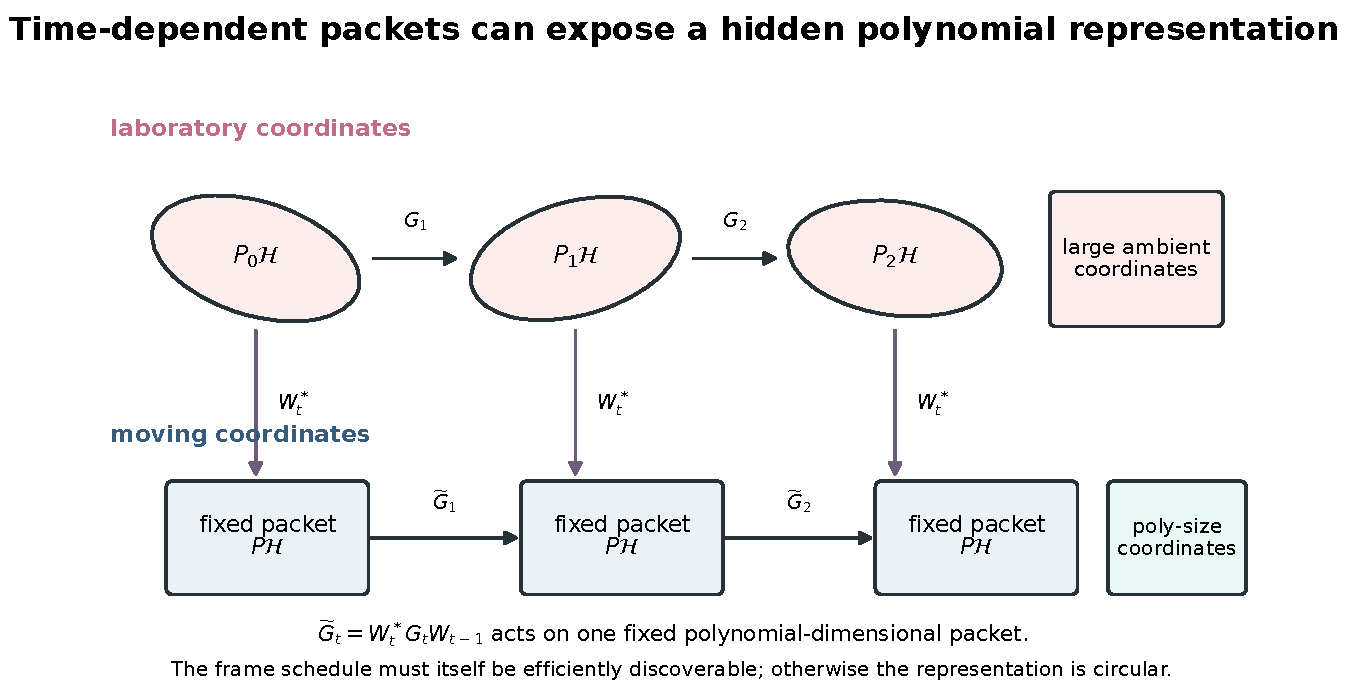
\includegraphics[width=.94\textwidth]{assets/s_moving_frame_packets.pdf}
\caption{A circuit may fail to preserve one laboratory-frame packet while remaining inside a small packet in a computable moving frame.}
\end{figure}

\subsection{Sparse packet-transfer graphs}
Let
\[
I=\sum_{\alpha\in\Lambda}P_\alpha
\]
be an orthogonal packet decomposition. Write the gate blocks as
\[
G_{t;\beta\alpha}=P_\beta G_tP_\alpha.
\]
Starting from an active packet set $S_0$, define recursively
\begin{equation}
S_t
=
\left\{
\beta:\exists\alpha\in S_{t-1}
\text{ with }G_{t;\beta\alpha}\ne0
\right\}.
\label{s:eq:reachable-packet-set}
\end{equation}

\begin{corollary}[Reachable packet-graph collapse]
\label{s:cor:packet-graph-collapse}
Suppose the packet sets $S_t$ and nonzero transfer blocks are computable in polynomial time, and
\[
D_t
=
\sum_{\alpha\in S_t}\rank P_\alpha
\le\poly(n)
\]
for every $t$. If all active block updates and the final measurement are efficiently computable, then the circuit family is classically polynomial-time simulable.
\end{corollary}

\begin{proof}
Take
\[
P_t=\sum_{\alpha\in S_t}P_\alpha.
\]
The definition of $S_t$ gives $G_tP_{t-1}=P_tG_tP_{t-1}$. Apply \cref{s:thm:moving-packet-collapse}.
\end{proof}

This theorem permits exact sector changes. What matters is not that one charge be fixed, but that the union of reachable sectors remain polynomial.

\begin{corollary}[Bounded-excitation collapse]
\label{s:cor:bounded-excitation-collapse}
Consider $n$ qubits and suppose the initial state and every circuit prefix are certified to lie in
\[
\Hh_{\le K}
=
\bigoplus_{k=0}^{K}\Hh_{n,k}
\]
for a fixed constant $K$. If initialization, the gate actions, and the measurement are computable in polynomial time in the occupation basis, then the circuit family lies in $P$, even when individual gates change excitation number.
\end{corollary}

\begin{proof}
The active dimension is
\[
\sum_{k=0}^{K}\binom nk
=O(n^K).
\]
Let $P$ project onto $\Hh_{\le K}$. By the hypothesis on the actual circuit prefixes, $P\psi_t=\psi_t$ at every step. Consequently $PG_tP\psi_{t-1}=G_t\psi_{t-1}$ on the evolving state, even if the gate does not preserve all of $P\Hh$. The restricted update therefore reproduces that trajectory exactly. The hypothesis supplies efficient initialization, updates, and measurement in these polynomially many coordinates.
\end{proof}

For example, a fixed-weight input followed by only a constant number of pair-creation or pair-annihilation events remains in a constant collection of low-weight sectors. Exact number conservation is therefore stronger than necessary.

\begin{figure}[H]
\centering
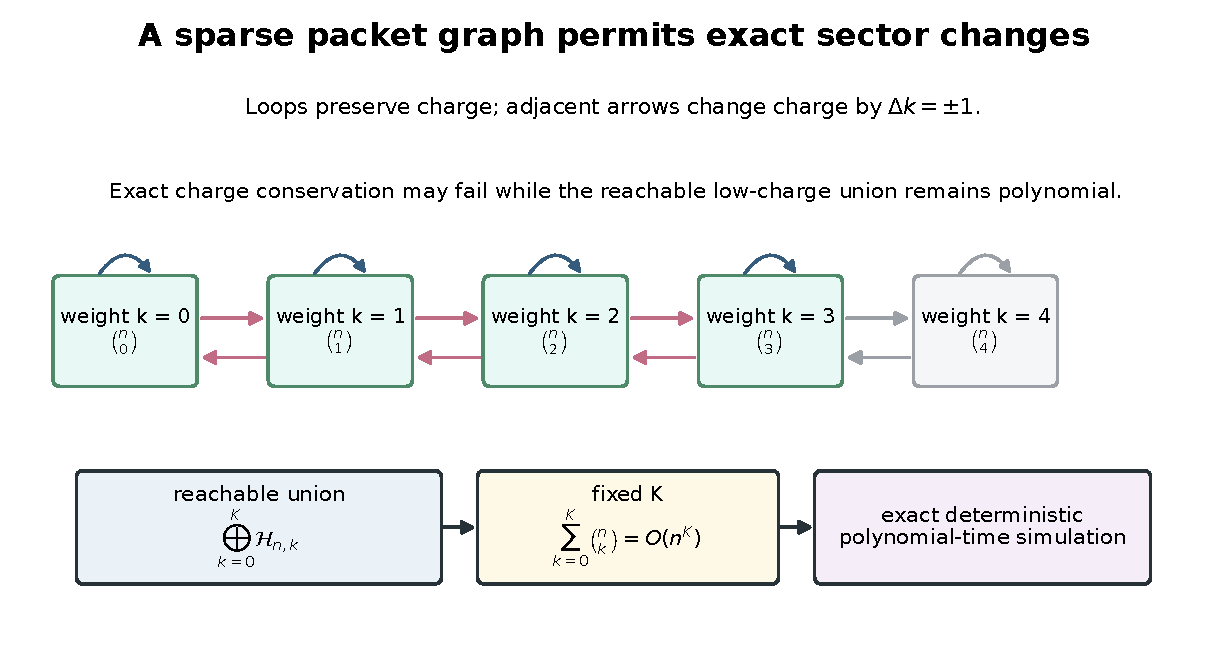
\includegraphics[width=.90\textwidth]{assets/s_reachable_packet_graph.pdf}
\caption{Sector-changing gates remain classically tractable when the reachable packet graph and total active dimension stay polynomial.}
\end{figure}

\subsection{Approximate dynamic packets}
Define the one-step leakage from the scheduled packet by
\[
\delta_t
=
\|(I-P_t)G_tP_{t-1}\|.
\]
Let
\[
\widehat G_t=P_tG_tP_{t-1}.
\]

\begin{theorem}[Dynamic sum-of-leakages bound]
\label{s:thm:dynamic-leakage}
For an initial unit vector in $P_0\Hh$,
\[
\left\|
G_m\cdots G_1\ket{\psi_0}
-
\widehat G_m\cdots\widehat G_1\ket{\psi_0}
\right\|
\le
\sum_{t=1}^{m}\delta_t.
\]
For any acceptance operator $0\le M\le I$, the corresponding acceptance probabilities differ by at most
\[
2\sum_{t=1}^{m}\delta_t.
\]
\end{theorem}

\begin{proof}
A telescoping expansion inserts $G_t-\widehat G_t$ at one time. On $P_{t-1}\Hh$ this difference equals $(I-P_t)G_tP_{t-1}$, while all other unitary or projected factors have norm at most one. Summing the operator norms proves the state bound. If $\psi$ and $\phi$ have norm at most one, then
\[
|\langle\psi,M\psi\rangle-\langle\phi,M\phi\rangle|
\le
(\|\psi\|+\|\phi\|)\|\psi-\phi\|
\le2\|\psi-\phi\|.
\]
\end{proof}

\begin{corollary}[Approximate moving-packet collapse]
If the scheduled dimensions and updates are polynomial and
\[
\sum_t\delta_t\le\frac1{\poly(n)},
\]
then, after ordinary promise-gap amplification, the circuit family remains deterministically classically simulable in polynomial time.
\end{corollary}

The result is conservative but fully composable. It extends the fixed-projector estimate of \cref{s:ch:approximate-symmetry} to moving frames and changing packet sets.


\subsection{An adaptive certificate from discarded state vectors}
The operator-norm leakage certificate is uniform over every input in a packet. An adaptive simulator can use a less expensive certificate that follows its actual approximate state. The discarded vector must be accounted for before any normalization.

\begin{theorem}[Adaptive discarded-state certificate]
\label{s:thm:adaptive-discarded-state}
Let $G_1,\ldots,G_m$ be unitary operators on a finite-dimensional Hilbert space, and let $\psi_0=\phi_0$ be a unit vector. At each step choose an orthogonal projector $P_t$, possibly as a function of the previously computed approximate states. Define
\[
\psi_t=G_t\psi_{t-1},\qquad
\phi_t=P_tG_t\phi_{t-1},\qquad
\eta_t=\|(I-P_t)G_t\phi_{t-1}\|.
\]
Then
\[
\|\psi_m-\phi_m\|\le\sum_{t=1}^m\eta_t.
\]
For an effect $0\le M\le I$,
\[
\left|\langle\psi_m,M\psi_m\rangle-\langle\phi_m,M\phi_m\rangle\right|
\le2\sum_{t=1}^m\eta_t.
\]
No renormalization of $\phi_t$ is performed. The second quadratic form is an unnormalized acceptance estimate.
\end{theorem}

\begin{proof}
Fix the projectors chosen during the particular run. Put $d_t=(I-P_t)G_t\phi_{t-1}$. Subtraction gives the exact recurrence
\[
\psi_t-\phi_t=G_t(\psi_{t-1}-\phi_{t-1})+d_t.
\]
Since $\psi_0-\phi_0=0$, iteration yields
\[
\psi_m-\phi_m=\sum_{t=1}^mG_m\cdots G_{t+1}d_t.
\]
Every unitary product preserves norm, so the triangle inequality proves the state estimate. Also $\|\psi_m\|=1$ and $\|\phi_m\|\le1$ because each projector is contractive. Expanding the difference of the two quadratic forms and using $\|M\|\le1$ gives the factor two. This proof applies to the chosen run even when the projectors were selected adaptively.
\end{proof}

\begin{example}[A rational two-step certificate]
Take
\[
G=\begin{pmatrix}3/5&-4/5\\4/5&3/5\end{pmatrix},
\qquad
P=\begin{pmatrix}1&0\\0&0\end{pmatrix},
\qquad
\psi_0=\phi_0=\begin{pmatrix}1\\0\end{pmatrix}.
\]
Using $G_1=G_2=G$ and $P_1=P_2=P$ gives
\[
\phi_2=\begin{pmatrix}9/25\\0\end{pmatrix},\qquad
\psi_2=\begin{pmatrix}-7/25\\24/25\end{pmatrix},\qquad
\eta_1=4/5,\quad\eta_2=12/25.
\]
The squared state error is $832/625$, below $(\eta_1+\eta_2)^2=1024/625$. The rational validation script checks these values exactly. The deliberately large tail illustrates a valid but loose certificate, not an efficient approximation.
\end{example}

The theorem closes global error accounting for any adaptive projection run whose discarded vectors or certified norm bounds can be computed. It does not prove that the retained representation stays polynomial, that the discarded norm is cheap to evaluate, or that a small tail can always be found. Those are separate algorithmic obligations. This is a written theorem with exact finite controls, not an additional Lean formalization.

\chapter{Exact symmetry families}
\section{Fixed charge and exact-number circuits}
\label{s:ch:fixed-charge}
\index{Hamming weight}
\index{particle number}

\subsection{Excitation-number packets}
For $n$ qubits, define
\[
\widehat N
=
\sum_{q=1}^n\frac{I-Z_q}{2}.
\]
Its eigenvalues are $k=0,1,\ldots,n$. The projector onto Hamming weight $k$ is
\[
P_{n,k}
=
\sum_{|x|=k}\ket x\bra x,
\]
and
\[
\dim P_{n,k}\Hh
=
\binom nk.
\]
The decomposition
\[
(\C^2)^{\otimes n}
=
\bigoplus_{k=0}^n\Hh_{n,k}
\]
recovers the full dimension through
\[
\sum_{k=0}^n\binom nk=2^n.
\]

\subsection{Number-preserving gates}
Single-qubit $R_Z$ gates commute with $\widehat N$. A two-qubit exchange rotation acts in the ordered basis $\ket{00},\ket{01},\ket{10},\ket{11}$ as
\[
U_{XY}(\theta,\phi)
=
\begin{pmatrix}
1&0&0&0\\
0&\cos\theta&-ie^{-i\phi}\sin\theta&0\\
0&-ie^{i\phi}\sin\theta&\cos\theta&0\\
0&0&0&1
\end{pmatrix}.
\]
It rotates $\ket{01}$ and $\ket{10}$ while fixing $\ket{00}$ and $\ket{11}$, so it preserves exact Hamming weight.

\begin{corollary}[Fixed-charge polynomial simulation]
\label{s:cor:fixed-charge-poly}
For every fixed $k$, a polynomial-time uniform family of number-preserving circuits initialized in $\Hh_{n,k}$ and measured by an efficiently computable observable is classically simulable in polynomial time, provided the initial weight-$k$ coordinates can be computed efficiently and each restricted local gate is efficiently applied in that basis.
\end{corollary}

\begin{proof}
For fixed $k$,
\[
\dim\Hh_{n,k}=\binom nk=O(n^k).
\]
The weight-$k$ basis is efficiently indexed by $k$-element subsets. A local number-preserving gate changes only basis states containing the affected occupation pattern. Apply \cref{s:thm:poly-packet}.
\end{proof}

\subsection{Sparse update structure}
A one-qubit diagonal phase changes one amplitude at a time. An exchange gate on modes $p,q$ couples a basis state only to the state obtained by moving one excitation between those modes. Thus every column of the restricted gate has at most two nonzero entries. For fixed $k$, the total update cost is polynomial in $n$.

\subsection{Uniformity and input encoding}
The fixed-charge corollary assumes $k$ is a fixed constant independent of $n$. It also applies when $k=O(1)$ is supplied by the circuit family. If $k$ is written in binary and allowed to scale as $n/2$, the sector can become exponential. The theorem is about the dimension and update cost of the actual active sector, not the name of the symmetry.

\begin{figure}[H]
\centering
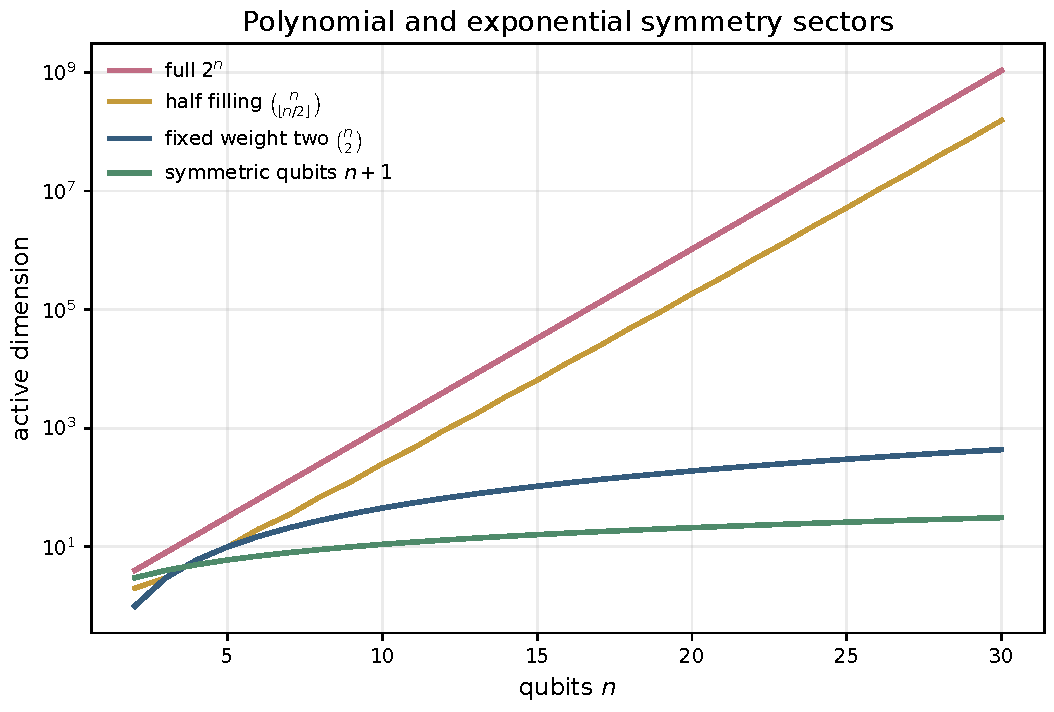
\includegraphics[width=.83\textwidth]{assets/s_dimension_scaling.pdf}
\caption{Fixed weight and permutation symmetry can be polynomial, while half filling remains exponential.}
\end{figure}

\subsection{Observables}
A diagonal observable depending on occupations is immediate. Few-body number-preserving observables are sparse in the subset basis. More global observables may require additional structure. The measurement hypothesis in \cref{s:thm:poly-packet} cannot be omitted: a compactly evolved state does not help if the requested output itself hides exponential work.

\section{The exact weight-two benchmark}
\label{s:ch:benchmarks}
\index{benchmark}

\subsection{Purpose and status}
The benchmark record compares a full state-vector simulator with a simulator restricted to the exact weight-two packet. Both use the same local gate arithmetic. The benchmark is not a hardware claim and not a universal performance model. It shows that the exact dimension reduction can translate into large memory and repeated-application gains in an ordinary implementation.

\begin{recordbox}
At $n=20$, the full state has $1{,}048{,}576$ amplitudes and the exact weight-two packet has $190$. The archived repeated-application gain is $958.8$, the one-shot gain is $54.8$, and the amplitude-memory ratio is $5518.8$. The recorded relative reconstruction error is zero at the displayed precision.
\end{recordbox}

\subsection{Recorded table}
\begin{longtable}{@{}rrrrrrr@{}}
\caption{Recorded exact-weight-two benchmark.}\label{s:tab:weight-two}\\
\toprule
$n$ & full dim. & packet dim. & apply gain & one-shot gain & memory gain & rel. error\\
\midrule
\endfirsthead
\toprule
$n$ & full dim. & packet dim. & apply gain & one-shot gain & memory gain & rel. error\\
\midrule
\endhead
8 & 256 & 28 & 1.11 & 1.64 & 9.14 & 0\\
10 & 1,024 & 45 & 1.51 & 2.02 & 22.8 & 0\\
12 & 4,096 & 66 & 2.95 & 3.98 & 62.1 & 0\\
14 & 16,384 & 91 & 8.55 & 11.0 & 180.0 & 0\\
16 & 65,536 & 120 & 33.0 & 36.9 & 546.1 & 0\\
18 & 262,144 & 153 & 131.3 & 39.1 & 1,713.4 & 0\\
20 & 1,048,576 & 190 & 958.8 & 54.8 & 5,518.8 & 0\\
\bottomrule
\end{longtable}

\subsection{What is machine independent}
The dimension identity
\[
\frac{2^n}{\binom n2}
\]
is independent of implementation. It predicts an exponential memory advantage for fixed $k=2$. The measured runtime ratio need not equal the dimension ratio. Packet indexing, compilation, sparse update kernels, allocation, and cache behavior determine the constant factors.

\subsection{Repeated application versus one shot}
Let $C_{\rm compile}$ be the cost of constructing the packet basis and restricted gate plans, and let $C_{\rm apply}$ be one packet application. Reusing the compiled plan $R$ times costs
\[
C_{\rm packet}(R)
=
C_{\rm compile}+RC_{\rm apply}.
\]
If the full path costs $RC_{\rm full}$, the packet method breaks even when
\[
R>
\frac{C_{\rm compile}}
{C_{\rm full}-C_{\rm apply}}.
\]
This is why time evolution, parameter sweeps, variational loops, and repeated likelihood evaluations are natural applications.

\begin{figure}[H]
\centering
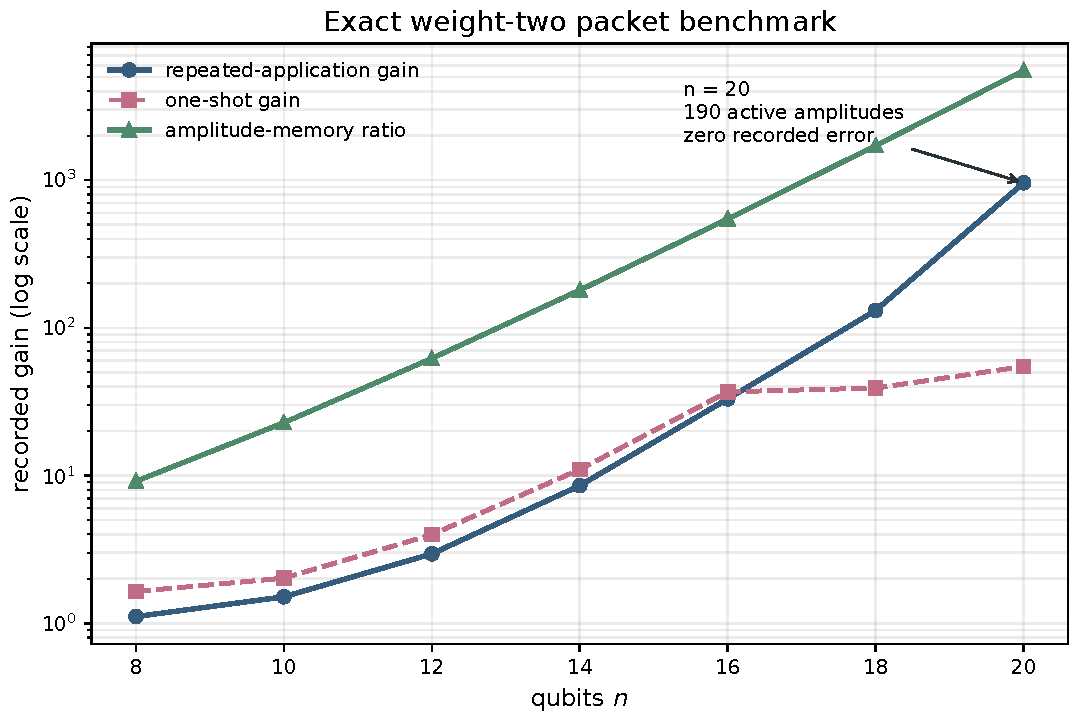
\includegraphics[width=.86\textwidth]{assets/s_weight_two_benchmark.pdf}
\caption{Recorded runtime and memory gains for the exact-weight-two packet.}
\end{figure}

\subsection{Independent reconstruction check}
The release code generates a random packet state, embeds it in the full Hilbert space, applies the same $R_Z$ and exchange gates through both arithmetic paths, and compares the final states. The representative checks at $(n,k)=(6,1),(8,2),(10,2)$ produce errors near machine precision.

\paragraph{Scope.}
The recorded benchmark supports exactness and implementation value for a symmetry-preserving subclass. It does not show that generic quantum circuits admit comparable reductions.

\section{Coarse packets and the honest limitation}
\label{s:ch:coarse-packets}

\subsection{Parity}
The even- and odd-parity packets each have dimension
\[
2^{n-1}.
\]
Parity removes half the state vector. This can produce a useful constant factor, but it does not change exponential scaling.

A pair-creation rotation mixes $\ket{00}$ and $\ket{11}$ and therefore changes excitation number by two while preserving parity. The packet is exact for a parity-preserving circuit, but its internal dimension remains exponential.

\subsection{Weight modulo four}
A four-qubit rotation between $\ket{0000}$ and $\ket{1111}$ changes excitation number by four. It can mix exact-weight sectors while preserving weight modulo four. A single residue packet contains asymptotically one quarter of all basis states. Again, the reduction is a constant factor.

\subsection{Half filling}
At half filling,
\[
\binom n{\lfloor n/2\rfloor}
\sim
\frac{2^n}{\sqrt{\pi n/2}}.
\]
The packet is smaller by a polynomial factor, but it remains exponential. At $n=20$, the half-filled packet contains $184{,}756$ amplitudes. The archived repeated-application gain is approximately $7.396$, while the one-shot gain is $0.6529$, meaning the packet path was slower in that single-run test after compilation overhead.

\begin{recordbox}
The half-filled benchmark demonstrates a necessary distinction: dimension reduction can be exact and useful without yielding polynomial complexity or a one-shot speedup.
\end{recordbox}

\begin{figure}[H]
\centering
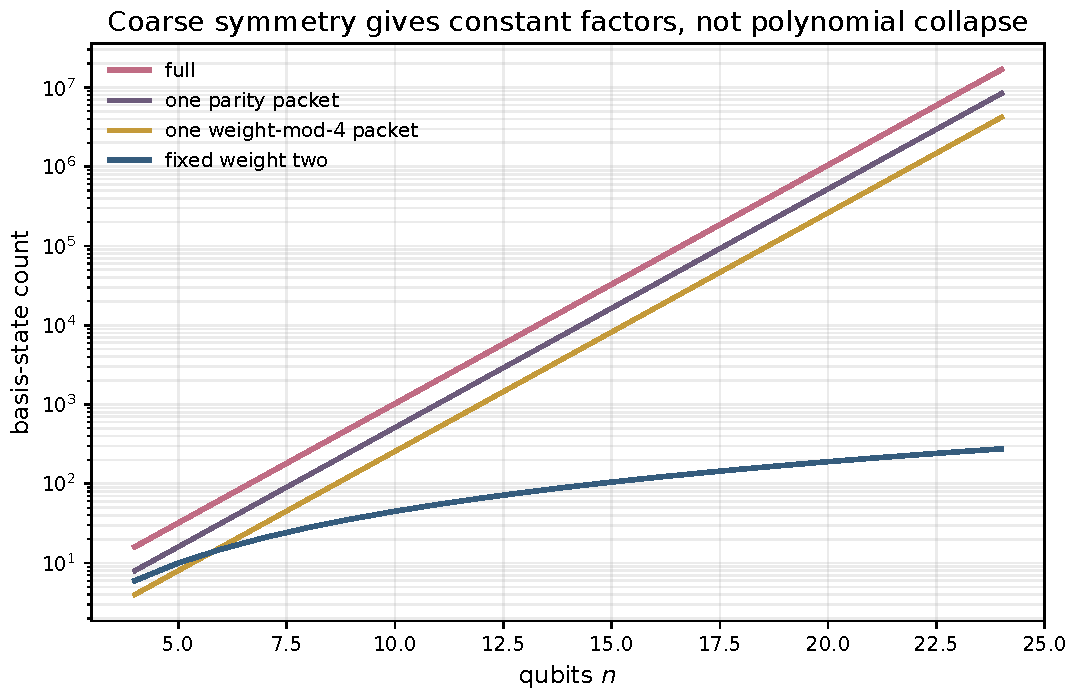
\includegraphics[width=.82\textwidth]{assets/s_coarse_vs_fine.pdf}
\caption{Parity and mod-four packets retain an exponential number of basis states.}
\end{figure}

\subsection{Entanglement inside a packet}
A small number of symmetry labels does not imply low entanglement. The half-filled packet can support volume-law entanglement. Tensor-network bond dimension and packet dimension are independent resources. A robust simulator should therefore track both
\[
(D_{\rm packet},\chi_{\rm internal}),
\]
where $\chi_{\rm internal}$ measures the cost of representing the state inside the packet.

\subsection{The no-label shortcut}
A stabilizer syndrome is only a label. A momentum quantum number is only a label. A total charge residue is only a label. The internal multiplicity space may still contain exponentially many degrees of freedom. The packet-simulation theorem becomes polynomial only when the complete active representation, not merely the label set, has polynomial classical cost.

\section{Permutation-symmetric circuits and Dicke coordinates}
\label{s:ch:permutation-symmetry}
\index{Dicke state}
\index{permutation symmetry}

\subsection{The symmetric subspace}
Let the symmetric group $S_n$ act by permuting the $n$ tensor factors. The fully symmetric qubit subspace is spanned by the Dicke states
\[
\ket{D_n^k}
=
\binom nk^{-1/2}
\sum_{|x|=k}\ket x,
\qquad
0\le k\le n.
\]
Its dimension is $n+1$.

\begin{derivedbox}
If the initial state is permutation symmetric with efficiently computable Dicke coordinates, every gate preserves the fully symmetric subspace, the gate matrices in the Dicke basis are computable in polynomial time, and the final measurement is permutation invariant and efficient, then the circuit family lies in $P$.
\end{derivedbox}

\begin{theorem}[Permutation-symmetric collapse]
\label{s:thm:permutation-collapse}
Under the hypotheses above, an $n$-qubit circuit can be simulated using an $(n+1)$-component classical state vector and polynomial-time updates.
\end{theorem}

\begin{proof}
The projector onto the trivial $S_n$ representation has rank $n+1$. The Dicke basis is explicitly indexed by $k=0,\ldots,n$. Apply \cref{s:thm:poly-packet}.
\end{proof}

\begin{figure}[H]
\centering
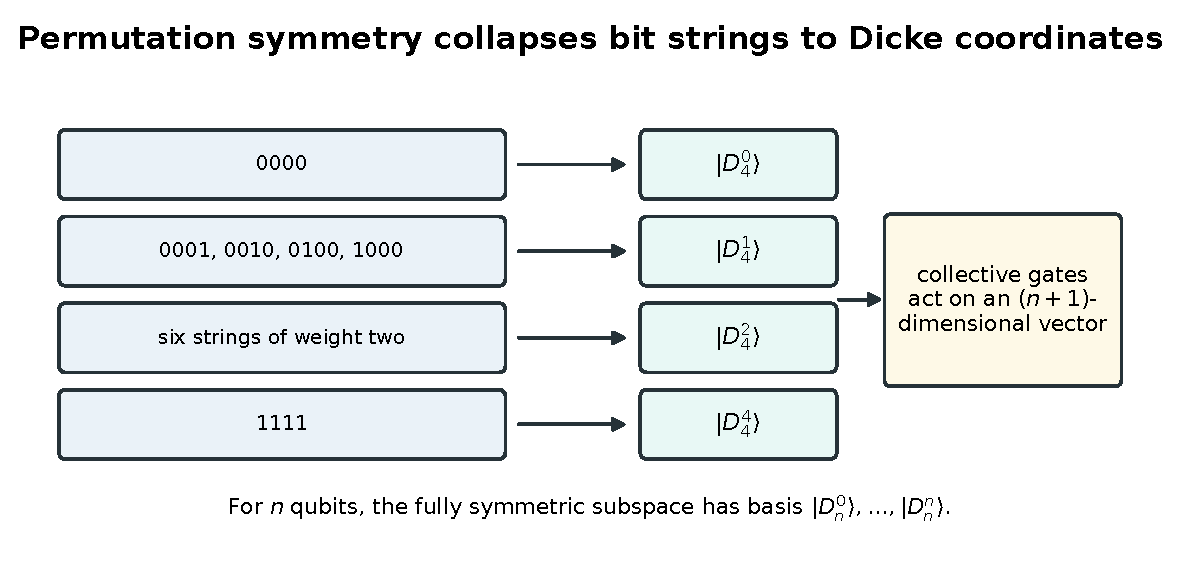
\includegraphics[width=.94\textwidth]{assets/s_dicke_basis.pdf}
\caption{Computational-basis orbits become Dicke coordinates.}
\end{figure}

\subsection{Collective spin operators}
Define
\[
J_a=\frac12\sum_{q=1}^n\sigma_a^{(q)},
\qquad a\in\{x,y,z\}.
\]
The operators $J_a$ preserve the symmetric subspace. We use the computational convention $\sigma_z\ket0=\ket0$ and $\sigma_z\ket1=-\ket1$. Thus $J_z\ket{D_n^k}=(n/2-k)\ket{D_n^k}$. For the following occupation formulas define $J_+=J_x-iJ_y$ and $J_-=J_x+iJ_y$, so that the subscript records increasing or decreasing excitation number rather than magnetic quantum number. Then
\[
J_+\ket{D_n^k}
=
\sqrt{(n-k)(k+1)}\ket{D_n^{k+1}},
\]
\[
J_-\ket{D_n^k}
=
\sqrt{k(n-k+1)}\ket{D_n^{k-1}}.
\]
Thus collective rotations and polynomial functions of collective spin admit banded or structured updates on $n+1$ amplitudes.

\subsection{Symmetric qudits}
For local dimension $d$, the symmetric subspace has occupation-number basis
\[
(n_1,\ldots,n_d),
\qquad
n_1+\cdots+n_d=n,
\]
and dimension
\begin{equation}
\dim\Sym^n(\C^d)
=
\binom{n+d-1}{d-1}.
\label{s:eq:symmetric-qudit-dim}
\end{equation}
For fixed $d$, this is polynomial in $n$.

\begin{corollary}[Fixed-local-dimension symmetric qudits]
A uniform family of fully symmetric $d$-level circuits is classically polynomial-time simulable for fixed $d$, provided its occupation-basis updates and measurement are polynomial-time computable.
\end{corollary}

\begin{figure}[H]
\centering
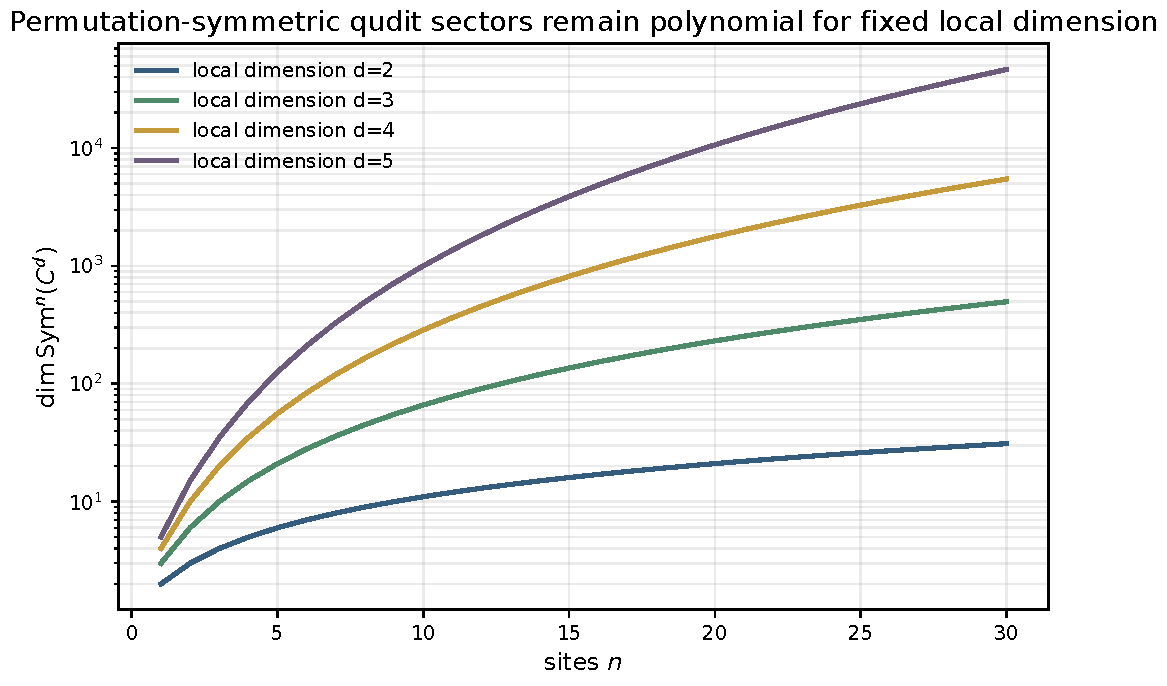
\includegraphics[width=.80\textwidth]{assets/s_symmetric_qudit_scaling.pdf}
\caption{Symmetric qudit sectors remain polynomial for every fixed local dimension.}
\end{figure}

\subsection{What full symmetry excludes}
A generic two-qubit gate acting on one selected pair does not preserve the fully symmetric subspace. Symmetry is preserved by collective gates or by circuits arranged so that the total operation commutes with all permutations. A gatewise packet simulator requires gatewise invariance, or else it must combine several elementary gates into a symmetry-preserving layer and audit intermediate leakage.

\section{Schur--Weyl coordinates and total-spin packets}
\label{s:ch:schur}
\index{Schur-Weyl duality}

\subsection{Decomposition}
For $n$ qudits of local dimension $d$, Schur--Weyl duality decomposes
\[
(\C^d)^{\otimes n}
\cong
\bigoplus_{\lambda\vdash n,\,\ell(\lambda)\le d}
\mathcal U_\lambda\otimes\mathcal V_\lambda,
\]
where $\mathcal U_\lambda$ carries an irreducible unitary-group representation and $\mathcal V_\lambda$ carries a symmetric-group representation. A permutation-invariant operator acts as
\[
A
=
\bigoplus_\lambda
A_\lambda\otimes I_{\mathcal V_\lambda}.
\]

The label $\lambda$ can be polynomially short even when the multiplicity space $\mathcal V_\lambda$ is exponentially large. This is a canonical example of the difference between a small packet label and a small active representation.

\subsection{Qubit total spin}
For qubits, the decomposition may be labeled by total spin $j$ and a multiplicity index. A collective $SU(2)$ operation acts nontrivially only on the $(2j+1)$-dimensional spin factor and as the identity on multiplicity. If the initial state and observable are insensitive to multiplicity, the effective dimension can be small. If arbitrary information is stored in multiplicity, total-spin labeling alone does not compress it.

\begin{principle}[Multiplicity audit]
A representation-theoretic packet must be recorded as
\[
\text{irrep label}
\quad+
\text{irrep carrier}
\quad+
\text{multiplicity space}.
\]
Dropping the multiplicity space is valid only when the dynamics, input, and measurement make it redundant.
\end{principle}

\subsection{Efficient Schur simulation regime}
A Schur-coordinate simulation is polynomial when the number of active partitions is polynomial, the retained carrier and multiplicity dimensions are polynomial or compactly represented, and each gate has an efficient action in these coordinates. Fully symmetric dynamics is the one-row partition and therefore the simplest case.

\subsection{Possible compiler use}
A symmetry compiler can detect collective layers, transform them into Schur coordinates, apply small representation matrices, and transform only when required. The transformation itself must be costed. In a purely classical simulator, one may never materialize the full Schur transform if the initial state is already specified by occupation or spin coordinates.

\begin{frontierbox}
A broad Schur-based collapse theorem requires explicit uniform algorithms for active-partition discovery, multiplicity handling, and local-gate updates. The decomposition alone is not the algorithm.
\end{frontierbox}

\section{Permutation-invariant mixed states and commutant compression}
\label{s:ch:commutant-collapse}
\index{commutant compression}
\index{permutation twirl}
\index{permutation-invariant density operator}

\subsection{Why multiplicity can disappear without being discarded}
The fully symmetric subspace is only one Schur--Weyl packet. A general permutation-invariant mixed state can occupy every Schur label while still admitting a polynomial classical description for fixed local dimension. The reason is that the exponentially large symmetric-group multiplicities occur as identity factors rather than independent dynamical coordinates.

Let $S_n$ act on
\[
\Hh_{n,d}=(\C^d)^{\otimes n}
\]
by permuting tensor factors. Schur--Weyl duality gives
\begin{equation}
\Hh_{n,d}
\cong
\bigoplus_{\lambda\vdash n,\,\ell(\lambda)\le d}
\mathcal U_\lambda\otimes\mathcal V_\lambda,
\label{s:eq:schur-decomp-commutant}
\end{equation}
where $S_n$ acts trivially on the first tensor factor and irreducibly on $\mathcal V_\lambda$.

\subsection{The permutation twirl}
Define the twirling channel
\begin{equation}
\mathcal T_n(X)
=
\frac1{n!}
\sum_{\pi\in S_n}
U_\pi XU_\pi^*.
\label{s:eq:permutation-twirl}
\end{equation}
Its image is the commutant of the permutation action.

\begin{lemma}[Invariant observables see only the twirl]
\label{s:lem:twirl-observable}
If $A$ commutes with every $U_\pi$, then
\[
\Tr(A\rho)
=
\Tr\bigl(A\mathcal T_n(\rho)\bigr)
\]
for every density operator $\rho$.
\end{lemma}

\begin{proof}
Using cyclicity of the trace and $U_\pi^*AU_\pi=A$,
\[
\Tr\bigl(A\mathcal T_n(\rho)\bigr)
=
\frac1{n!}\sum_\pi
\Tr(AU_\pi\rho U_\pi^*)
=
\frac1{n!}\sum_\pi
\Tr(U_\pi^*AU_\pi\rho)
=
\Tr(A\rho).
\]
\end{proof}

If a unitary $U$ and acceptance operator $M$ are permutation invariant, then $U^*MU$ is invariant. Therefore the final probability depends on the input only through its twirl. This permits an observable-specific collapse even when the original pure input is not itself symmetric.

\subsection{Exact commutant record}
Let
\[
u_\lambda=\dim\mathcal U_\lambda,
\qquad
f_\lambda=\dim\mathcal V_\lambda.
\]
Schur's lemma gives the following normal form.

\begin{lemma}[Permutation-invariant state normal form]
\label{s:lem:invariant-state-normal-form}
A density operator $\rho$ commutes with every permutation if and only if it can be written as
\begin{equation}
\rho
=
\bigoplus_\lambda
p_\lambda\,\rho_\lambda\otimes
\frac{I_{\mathcal V_\lambda}}{f_\lambda},
\label{s:eq:commutant-state-record}
\end{equation}
where $p_\lambda\ge0$, $\sum_\lambda p_\lambda=1$, and each $\rho_\lambda$ is a density operator on $\mathcal U_\lambda$ whenever $p_\lambda>0$. The weights $p_\lambda$ and the unnormalized blocks $p_\lambda\rho_\lambda$ are unique. The normalized block $\rho_\lambda$ is unique only when $p_\lambda>0$ and is omitted when $p_\lambda=0$.
\end{lemma}

The complete state record is therefore
\[
\left\{
(p_\lambda,\rho_\lambda)
\right\}_\lambda.
\]
The multiplicity dimension $f_\lambda$ affects normalization and degeneracy, but no $f_\lambda\times f_\lambda$ matrix needs to be stored.

A permutation-invariant unitary has the form
\begin{equation}
U
=
\bigoplus_\lambda
U_\lambda\otimes I_{\mathcal V_\lambda},
\label{s:eq:commutant-unitary-form}
\end{equation}
and a permutation-invariant measurement operator has the analogous form
\[
M
=
\bigoplus_\lambda
M_\lambda\otimes I_{\mathcal V_\lambda}.
\]
The output probability is
\begin{equation}
\Tr(MU\rho U^*)
=
\sum_\lambda
p_\lambda
\Tr\bigl(M_\lambda U_\lambda\rho_\lambda U_\lambda^*\bigr).
\label{s:eq:commutant-output}
\end{equation}

\subsection{Polynomial parameter bound}
The number of partitions of $n$ with at most $d$ parts is bounded by the number of weak compositions:
\[
\#\{\lambda:\ell(\lambda)\le d\}
\le
\binom{n+d-1}{d-1}
=O_d(n^{d-1}).
\]
The Weyl dimension formula gives
\begin{equation}
u_\lambda
=
\prod_{1\le i<j\le d}
\frac{\lambda_i-\lambda_j+j-i}{j-i}
=O_d\left(n^{d(d-1)/2}\right).
\label{s:eq:weyl-dimension-bound}
\end{equation}
Therefore
\begin{equation}
\sum_\lambda u_\lambda^2
=O_d\left(n^{d^2-1}\right).
\label{s:eq:commutant-parameter-bound}
\end{equation}

\begin{theorem}[Schur-commutant collapse]
\label{s:thm:schur-commutant-collapse}
Fix the local dimension $d$. Consider a polynomial-time uniform family of permutation-invariant quantum circuits or channels on $n$ qudits. Suppose:
\begin{enumerate}
\item the Schur-block record of the twirled input can be constructed in polynomial time;
\item the induced update on the invariant operator record in \cref{s:eq:commutant-state-record} is computable to polynomial precision in polynomial time;
\item the final measurement is permutation invariant and its Schur blocks are efficiently computable.
\end{enumerate}
Then the associated decision problem belongs to $P$.
\end{theorem}

\begin{proof}
Permutation covariance keeps the density operator inside the commutant algebra. By \cref{s:eq:commutant-parameter-bound}, that algebra has polynomial dimension for fixed $d$. The hypotheses supply polynomial-time initialization, updates, and measurement on this record. Apply \cref{s:thm:compressed-packet}.
\end{proof}

\begin{derivedbox}
For fixed local dimension, permutation-invariant mixed-state dynamics can be classically polynomial even when the state has support across exponentially large symmetric-group multiplicity spaces. Those multiplicities are exact identity factors in the invariant operator record.
\end{derivedbox}

\subsection{Qubit corollary}
For qubits, Schur labels are total spins $j$. The carrier dimension is
\[
u_j=2j+1\le n+1,
\]
and there are at most $\lfloor n/2\rfloor+1$ labels. Hence
\begin{equation}
\sum_j(2j+1)^2=O(n^3).
\label{s:eq:qubit-commutant-size}
\end{equation}

\begin{corollary}[Permutation-invariant qubit channels]
\label{s:cor:perm-invariant-qubit-channels}
A uniform permutation-covariant qubit channel family with efficiently computable total-spin block updates, efficiently available twirled input blocks, and a permutation-invariant measurement is classically simulable using $O(n^3)$ density-matrix parameters, up to constant factors and numerical precision.
\end{corollary}

Collective Hamiltonians that are polynomial expressions in $J_x,J_y,J_z$ are a basic test class because their total-spin matrices can be generated directly without constructing the full $2^n\times2^n$ operator.

\begin{figure}[H]
\centering
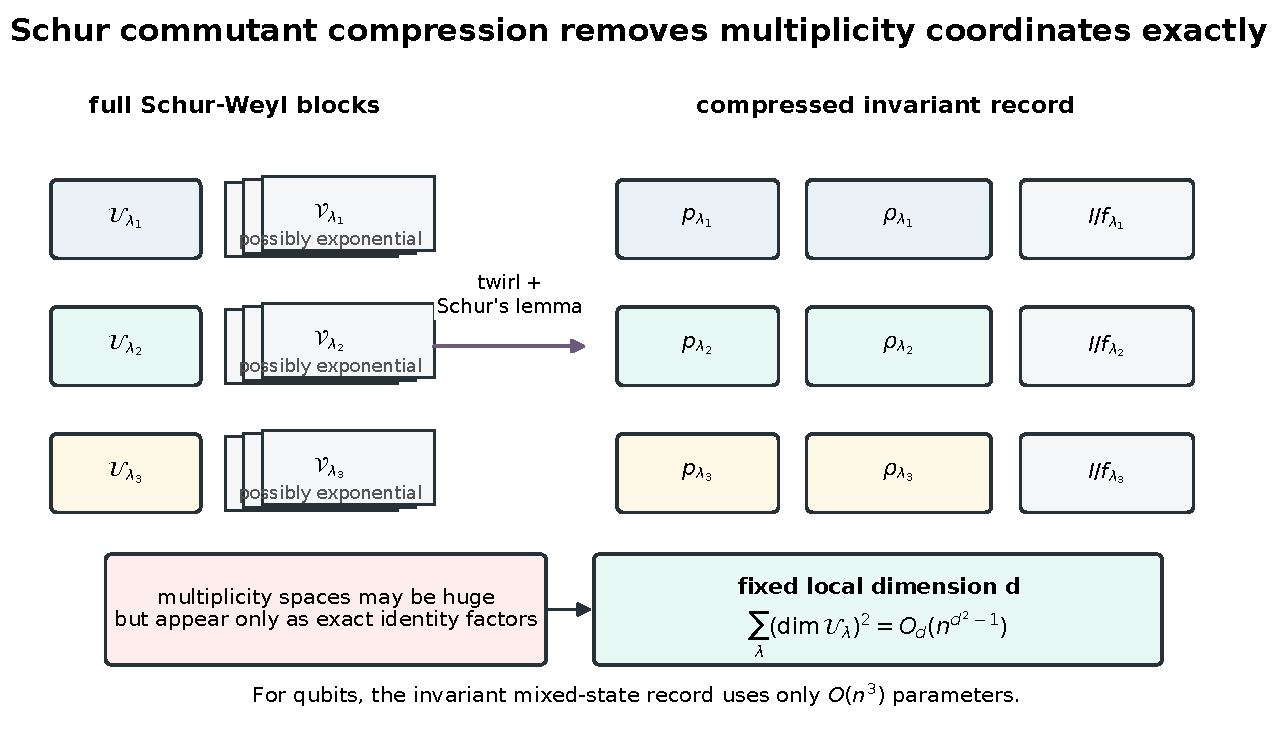
\includegraphics[width=.94\textwidth]{assets/s_schur_commutant_compression.pdf}
\caption{Permutation-invariant density operators retain the polynomial carrier blocks and replace each possibly exponential multiplicity space by an exact identity factor.}
\end{figure}

\subsection{What this theorem does not cover}
The theorem does not make an arbitrary local circuit easy. A gate acting on one selected pair generally fails to commute with all permutations. An arbitrary input may have Schur blocks that are difficult to compute from its succinct description. A non-invariant measurement can read information stored in multiplicity coordinates. Finally, allowing local dimension $d$ to grow with $n$ can make the commutant record superpolynomial.

The result is therefore a complete collapse theorem for a declared symmetry and access model, not a claim that Schur--Weyl decomposition alone solves generic many-body simulation.

\section{Orbit-quotient quantum walks}
\label{s:ch:orbit-quotients}
\index{quantum walk}
\index{orbit quotient}

\subsection{Orbit states}
Let a group $G$ act by automorphisms on a finite graph with vertex set $V$. The orbits are $\mathcal O_1,\ldots,\mathcal O_r$. Define normalized orbit states
\[
\ket{\mathcal O_a}
=
\frac1{\sqrt{|\mathcal O_a|}}
\sum_{x\in\mathcal O_a}\ket x.
\]
If the adjacency or Hamiltonian $H$ commutes with the group action, the span of these states is invariant whenever the partition is equitable.

The quotient matrix is
\[
\widetilde H_{ab}
=
\bra{\mathcal O_a}H\ket{\mathcal O_b}.
\]

\begin{theorem}[Orbit-quotient collapse]
\label{s:thm:orbit-collapse}
Suppose a uniformly described quantum walk has a polynomial number $r(n)$ of relevant orbits, an orbit-uniform initial state, an orbit-invariant final measurement, and polynomial-time algorithms for orbit sizes, quotient entries, initial orbit coordinates, and the restricted final measurement. For continuous-time evolution, also assume a polynomial bound on $|t|\|\widetilde H\|$ and efficient entry access to the precision required by the simulation. Then the walk can be simulated classically in polynomial time by the $r(n)\times r(n)$ quotient dynamics.
\end{theorem}

\begin{proof}
The orbit-state span is invariant. The state is represented by $r(n)$ amplitudes. Polynomial-time computation of quotient entries and ordinary polynomial-precision linear algebra satisfy \cref{s:thm:poly-packet}.
\end{proof}

\subsection{Hypercube example}
The $n$-dimensional hypercube is invariant under coordinate permutations. Its vertex orbits are Hamming-weight layers $0,1,\ldots,n$. In the normalized orbit basis, the quotient adjacency has couplings
\begin{equation}
\bra{k+1}A\ket{k}
=
\sqrt{(k+1)(n-k)}.
\label{s:eq:hypercube-coupling}
\end{equation}
Thus a walk on $2^n$ vertices initialized at $0^n$ evolves in an $(n+1)$-dimensional subspace.

\begin{figure}[H]
\centering
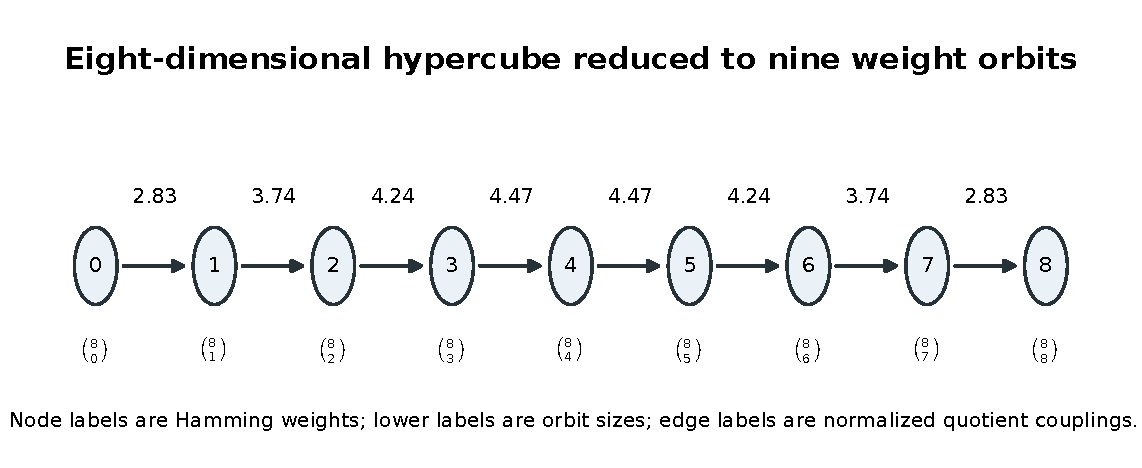
\includegraphics[width=.94\textwidth]{assets/s_hypercube_quotient.pdf}
\caption{The hypercube walk collapses to a weighted path of Hamming-weight orbits.}
\end{figure}

\subsection{The succinct-input caveat}
If the full graph is supplied explicitly, a polynomial-in-$|V|$ algorithm may still be exponential in the succinct parameter $n$. The theorem requires quotient data computable directly from the succinct graph description. Discovering graph automorphisms or orbit partitions can itself be difficult. For regular families such as hypercubes, Johnson graphs, association schemes, and Cayley graphs with known character theory, the quotient is explicit.

\subsection{Fourier packets}
On a cycle, translation characters diagonalize the adjacency operator. The continuous-time walk
\[
\ket{\psi(t)}=e^{-itA}\ket0
\]
is a sum of Fourier-character packets. This is the same discrete Fourier transform that appears as a signal-processing coordinate change, a group-character decomposition, and a quantum basis transformation.

\section{Few bosons and few fermions}
\label{s:ch:few-particles}
\index{boson}
\index{fermion}

\subsection{Bosonic occupation space}
For $N$ indistinguishable bosons in $m$ modes, a Fock basis state is an occupation vector
\[
(n_1,\ldots,n_m),
\qquad
n_1+\cdots+n_m=N.
\]
The dimension is
\begin{equation}
D_{\rm boson}(m,N)
=
\binom{N+m-1}{N}.
\label{s:eq:boson-dim}
\end{equation}
For fixed $N$, this is $O(m^N)$.

\subsection{Fermionic occupation space}
For $N$ fermions in $m$ modes, each mode is occupied at most once and
\begin{equation}
D_{\rm fermion}(m,N)
=
\binom mN.
\label{s:eq:fermion-dim}
\end{equation}
For fixed $N$, this is also polynomial in $m$.

\begin{corollary}[Few-particle collapse]
A polynomial-size number-preserving bosonic or fermionic circuit with a fixed number of particles is classically polynomial-time simulable if its initial occupation coordinates, mode-gate updates, and final observable are computable in polynomial time in the occupation basis.
\end{corollary}

\begin{proof}
Use \cref{s:eq:boson-dim,s:eq:fermion-dim} and \cref{s:thm:poly-packet}.
\end{proof}

\begin{figure}[H]
\centering
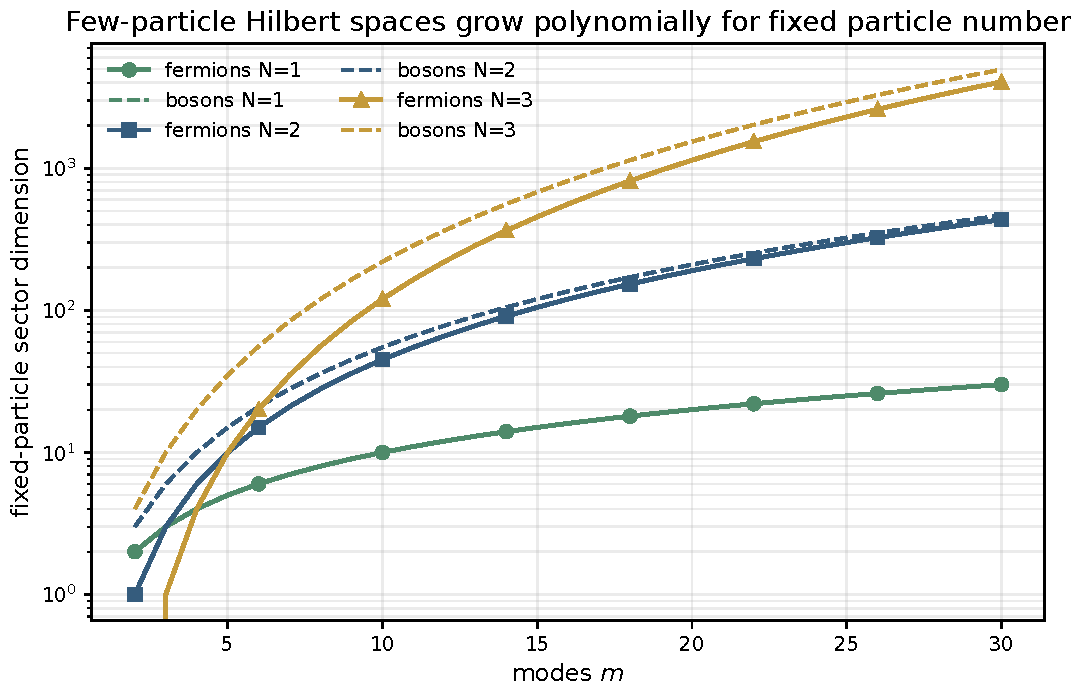
\includegraphics[width=.82\textwidth]{assets/s_few_particle_dimensions.pdf}
\caption{Fixed-particle bosonic and fermionic sectors grow polynomially with the number of modes.}
\end{figure}

\subsection{Gate updates}
A number-preserving one-body unitary acts on mode creation operators by
\[
a_i^\dagger
\longmapsto
\sum_j U_{ji}a_j^\dagger.
\]
A generic dense mode transformation can induce many occupation-basis transitions, but for fixed $N$ the basis dimension remains polynomial. Local hopping and phase gates are sparse. Few-body interactions remain polynomial to apply for fixed $N$, although the exponent can grow with $N$.

\subsection{Where the theorem stops}
If $N$ scales linearly with $m$, both dimensions become exponential. The fixed-number symmetry still reduces the full Fock space, but it does not prove polynomial simulation. Boson-sampling-type interference also shows that a fixed total particle number is not enough when the particle count itself scales with input size and the output asks for detailed many-body amplitudes.

\begin{scopebox}
The corollary is a fixed-particle theorem. It is not a claim that general many-boson or many-fermion quantum dynamics are classically easy.
\end{scopebox}

\section{Scaling phase diagrams for charge, particles, and local dimension}
\label{s:ch:scaling-phases}
\index{particle-number scaling}
\index{quasipolynomial simulation}
\index{subexponential simulation}

\subsection{Exact sector size is a complexity phase variable}
The statement ``fixed particle number is polynomial'' has a sharp extension. Let the particle number depend on the system size:
\[
k=k(n).
\]
The explicit-amplitude simulation cost of one fermionic or qubit weight packet is governed by
\[
D_{n,k}=\binom nk.
\]
For $1\le k\le n$, the standard bounds
\begin{equation}
\left(\frac nk\right)^k
\le
\binom nk
\le
\left(\frac{en}{k}\right)^k
\label{s:eq:binomial-basic-bounds}
\end{equation}
show that the growth changes continuously between polynomial and exponential regimes.

Because
\[
\binom nk=\binom n{n-k},
\]
write
\[
r(n)=\min\{k(n),n-k(n)\}.
\]

\begin{theorem}[Explicit fixed-charge phase diagram]
\label{s:thm:charge-phase-diagram}
For explicit amplitude storage in a weight-$k(n)$ packet:
\begin{enumerate}
\item the packet dimension is polynomial in $n$ if $r(n)=O(1)$;
\item the packet dimension is superpolynomial whenever $r(n)\to\infty$;
\item if $r(n)=O(\log n)$, then
\[
D_{n,k}=2^{O((\log n)^2)},
\]
so the explicit packet simulation is quasipolynomial;
\item if $r(n)=O(n^\alpha)$ for a fixed $0<\alpha<1$, then
\[
D_{n,k}=2^{O(n^\alpha\log n)},
\]
which is subexponential;
\item if $k(n)/n\to p\in(0,1)$, then
\[
\log_2 D_{n,k}
=
nH_2(k(n)/n)+O(\log n)
=
nH_2(p)+o(n),
\]
where $H_2$ is binary entropy, and the packet remains exponential.
\end{enumerate}
\end{theorem}

\begin{proof}
The upper bounds follow from \cref{s:eq:binomial-basic-bounds}. If $r=O(1)$, then $\binom nr=O(n^r)$. Conversely, suppose $r\to\infty$ and $r\le n/2$. If $r\le\sqrt n$, then
\[
\log\binom nr
\ge
r\log(n/r)
\ge
\frac r2\log n,
\]
whose ratio to $\log n$ diverges. If $r>\sqrt n$, then
\[
\log\binom nr
\ge
r\log2
\ge
\sqrt n\log2,
\]
which also dominates every constant multiple of $\log n$. For the final assertion, $p_n=k(n)/n$ stays in a compact subinterval of $(0,1)$. Stirling's formula gives
\[
\log_2\binom n{k(n)}
=nH_2(p_n)-\frac12\log_2\!\bigl(2\pi n p_n(1-p_n)\bigr)+O(1/n).
\]
The logarithmic term is $O(\log n)$, uniformly on that subinterval. Continuity of $H_2$ gives $nH_2(p_n)=nH_2(p)+o(n)$. Replacing $p_n$ by its limit inside an $O(\log n)$ estimate would require a convergence rate, which is not assumed here.
\end{proof}

\begin{derivedbox}
For the explicit occupation-amplitude representation, ``few particles'' means a bounded number of particles or holes. A slowly growing charge can still improve on full state-vector scaling, but it no longer guarantees membership in $P$.
\end{derivedbox}

\subsection{A bounded-excitation hierarchy}
The union of the first $K$ weight sectors has dimension
\[
D_{\le K}(n)
=
\sum_{k=0}^{K}\binom nk.
\]
For fixed $K$,
\[
D_{\le K}(n)=O(n^K).
\]
If $K=O(\log n)$, the same union is quasipolynomial. This refines \cref{s:cor:bounded-excitation-collapse}: bounded symmetry breaking preserves polynomial simulation, while logarithmically growing excitation gives a controlled quasipolynomial regime.

\subsection{Bosonic and fermionic analogues}
For $N$ fermions in $m$ modes,
\[
D_{\mathrm F}(m,N)=\binom mN.
\]
For $N$ bosons in $m$ modes,
\[
D_{\mathrm B}(m,N)=\binom{m+N-1}{N}.
\]
The same binomial analysis gives:

\begin{corollary}[Few-particle scaling]
\label{s:cor:few-particle-scaling}
With the number of modes as the input-size parameter:
\begin{enumerate}
\item fixed $N$ gives polynomial explicit-amplitude simulation;
\item $N=O(\log m)$ gives quasipolynomial sector size;
\item $N=O(m^\alpha)$, $0<\alpha<1$, gives subexponential sector size;
\item finite-density fermionic sectors remain exponential.
\end{enumerate}
For bosons, the statements hold in the dilute regime with the same occupation-basis access assumptions.
\end{corollary}

The adjective ``polynomial'' here refers to the sector dimension and efficient gate action. It does not assert that every interacting Hamiltonian has efficiently computable matrix elements or that every compact description remains closed.

\subsection{Symmetric qudits with growing local dimension}
The symmetric $d$-level subspace has dimension
\[
S(n,d)
=
\binom{n+d-1}{d-1}.
\]
For fixed $d$, this is polynomial in $n$. If $d=d(n)$ grows, the same phase transition appears.

\begin{proposition}[Growing-local-dimension boundary]
\label{s:prop:growing-d-boundary}
In the explicit occupation basis:
\begin{enumerate}
\item fixed $d$ gives $S(n,d)=O(n^{d-1})$;
\item $d=O(\log n)$ gives $S(n,d)=2^{O((\log n)^2)}$;
\item unbounded $d$ is not covered by the fixed-$d$ polynomial-collapse theorem without an additional internal compression.
\end{enumerate}
\end{proposition}

Thus permutation symmetry removes the exponential tensor-product multiplicity only when the number of local levels is controlled, or when the occupation record itself admits a second compression.

\begin{figure}[H]
\centering
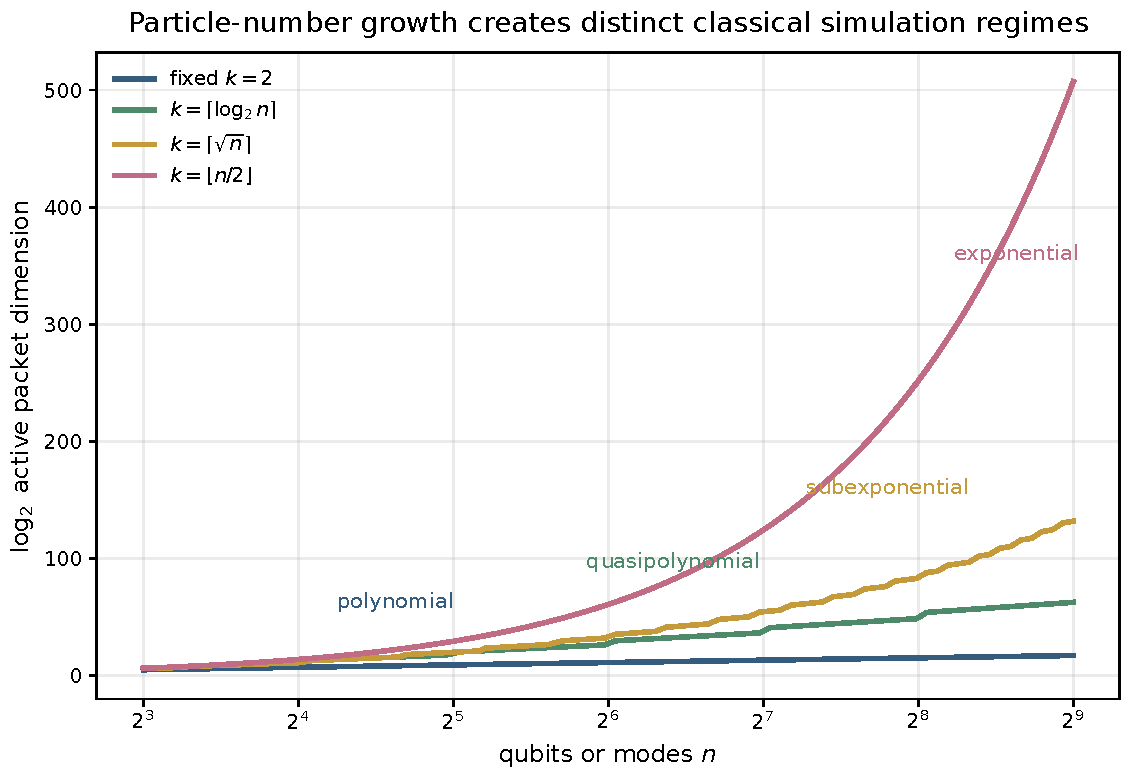
\includegraphics[width=.94\textwidth]{assets/s_particle_scaling_phases.pdf}
\caption{The active dimension passes through polynomial, quasipolynomial, subexponential, and exponential regimes as particle number grows.}
\end{figure}

\subsection{Complexity class versus practical runtime}
A polynomial sector can still have a large exponent. Fixed $k=20$ gives $O(n^{20})$ explicit amplitudes, which is in $P$ but may be impractical. Conversely, a subexponential sector may be useful at moderate size without changing the formal complexity class.

A complete performance claim should therefore report both:
\[
\text{asymptotic class}
\qquad\text{and}\qquad
\text{actual representation size and update cost}.
\]
This is why the benchmark chapters keep wall-clock evidence separate from the dimension theorems.

\section{Stabilizer syndromes and Clifford packets}
\label{s:ch:stabilizer}
\index{stabilizer}
\index{Clifford circuit}

\subsection{Syndrome projectors}
Let $S_1,\ldots,S_m$ be commuting Pauli stabilizers with eigenvalues $\pm1$. A syndrome $s\in\{0,1\}^m$ defines
\[
P_s
=
\prod_{j=1}^m
\frac{I+(-1)^{s_j}S_j}{2}.
\]
These projectors are orthogonal and sum to the identity. Syndrome measurement selects one packet, while recovery applies a syndrome-dependent transfer toward the code packet.

\subsection{The syndrome label is not the logical state}
If the code encodes $k$ logical qubits, a fixed syndrome packet can have dimension $2^k$. The syndrome has only $m$ bits, but arbitrary logical information remains inside the packet. Syndrome packetization therefore does not by itself prove efficient simulation.

\subsection{Tableau compression}
Clifford circuits provide a different route. A stabilizer state may occupy exponentially many computational-basis strings, yet it is represented by a polynomial-size stabilizer tableau. Clifford gates update the tableau in polynomial time, and Pauli measurements are efficiently computable. This is an example of the compressed-packet theorem rather than a small-dimensional packet theorem.

\begin{derivedbox}
Packet labels and internal encoding are complementary. A Clifford circuit restricted to selected syndromes may be simulated by a tableau augmented with the active syndrome graph, even when the packet dimensions are exponential.
\end{derivedbox}

\subsection{Non-Clifford residues}
A few non-Clifford gates can be handled by stabilizer decompositions, quasiprobability expansions, or magic-state rank methods. The cost grows with a non-Clifford resource such as stabilizer rank or robustness. Symmetry packets may reduce the number of relevant branches, but they do not eliminate the intrinsic cost of the non-Clifford residue.

\subsection{Error-correction interpretation}
The packet view separates three objects:
\[
\text{syndrome label},
\qquad
\text{logical state},
\qquad
\text{recovery transfer}.
\]
This separation is useful for compressed simulation of fault-tolerant protocols, but a full complexity statement must include repeated measurements, classical control, and the size of the logical state.

\section{Gaussian, fermionic, and matchgate compression}
\label{s:ch:gaussian}
\index{Gaussian circuit}
\index{matchgate}

\subsection{Polynomial covariance representations}
Gaussian bosonic and fermionic states are specified by first and second moments rather than by all Fock-basis amplitudes. A bosonic covariance matrix has size polynomial in the number of modes, and a fermionic Gaussian state is represented by an antisymmetric Majorana covariance matrix. Gaussian unitaries act by symplectic or orthogonal transformations:
\[
\Gamma\longmapsto S\Gamma S^T
\quad\text{or}\quad
\Gamma\longmapsto O\Gamma O^T.
\]
This is a compact internal encoding even when the corresponding Hilbert-space packet is exponentially large.

\subsection{Hybrid symmetry and Gaussianity}
Number conservation, parity, translation symmetry, and point-group symmetry can further block the covariance matrices. A simulator can therefore combine two reductions:
\[
\text{symmetry packetization}
+
\text{Gaussian internal encoding}.
\]
The first removes unreachable sectors. The second compresses states within the remaining sectors.

\subsection{Matchgate circuits}
Nearest-neighbor matchgate circuits have polynomial classical representations through fermionic Gaussian dynamics. Geometry matters: adding SWAP, fermionic SWAP, long-range gates, or a non-matchgate resource changes the simulation problem. A symmetry-collapse atlas should therefore record the gate library and connectivity as part of the model, not as implementation details.

\subsection{Low-rank non-Gaussian corrections}
One research direction is to represent a weakly non-Gaussian state as
\[
\rho
=
\sum_{a=1}^R c_a\rho_a^{\rm Gauss}
\]
with small Gaussian rank $R$, or as a Gaussian reference plus sparse packet corrections. A polynomial collapse requires $R$ and the update cost to remain polynomial.

\begin{frontierbox}
Gaussianity is an internal representation class, not a symmetry projector. A complete hybrid theorem must prove closure of the chosen compressed class under every allowed gate and bound the growth of any non-Gaussian residue.
\end{frontierbox}

\subsection{Few-particle versus Gaussian routes}
Fixed-particle simulation and Gaussian simulation are independent. A fixed two-fermion state may be non-Gaussian but live in a polynomial-dimensional sector. A half-filled Gaussian state may live in an exponential number sector but have a polynomial covariance description. The two-axis model in \cref{s:ch:compressed-packets} is designed to capture this distinction.

\chapter{States, measurements, and open dynamics}
\section{Density operators: populations and coherences}
\label{s:ch:density}
\index{density operator}
\index{coherence}

\subsection{Two packet indices}
A pure state uses one packet label. A density operator uses two:
\[
\rho
=
\sum_{\alpha,\beta}
P_\alpha\rho P_\beta.
\]
The diagonal block $P_\alpha\rho P_\alpha$ is population inside packet $\alpha$. The off-diagonal block $P_\alpha\rho P_\beta$ is coherence between packets $\alpha$ and $\beta$.

Discarding off-diagonal blocks is not merely a change of coordinates. It is a physical operation such as dephasing. An exact simulator must preserve all coherence blocks relevant to the final observable.

\subsection{Hilbert--Schmidt decomposition}
Orthogonality of the left-right operator packets gives
\[
\|\rho\|_2^2
=
\sum_{\alpha,\beta}
\|P_\alpha\rho P_\beta\|_2^2.
\]
This identity supplies an exact coherence-energy ledger. It can be used to decide which blocks are large, to audit dephasing, or to bound truncation errors in approximate packet simulations.

\subsection{Symmetry-preserving unitary dynamics}
If $U$ commutes with every packet projector, then
\[
P_\alpha U\rho U^\dagger P_\beta
=
U(P_\alpha\rho P_\beta)U^\dagger.
\]
The left and right packet labels are preserved. Populations and coherences evolve independently by their declared labels.

\subsection{Observable sparsity}
For an observable $M$,
\[
\Tr(M\rho)
=
\sum_{\alpha,\beta}
\Tr(P_\beta M P_\alpha\,P_\alpha\rho P_\beta).
\]
Only operator packets coupled by $M$ contribute. A measurement that is diagonal in the symmetry labels depends only on populations. A phase-sensitive measurement can require off-diagonal coherences.

\begin{figure}[H]
\centering
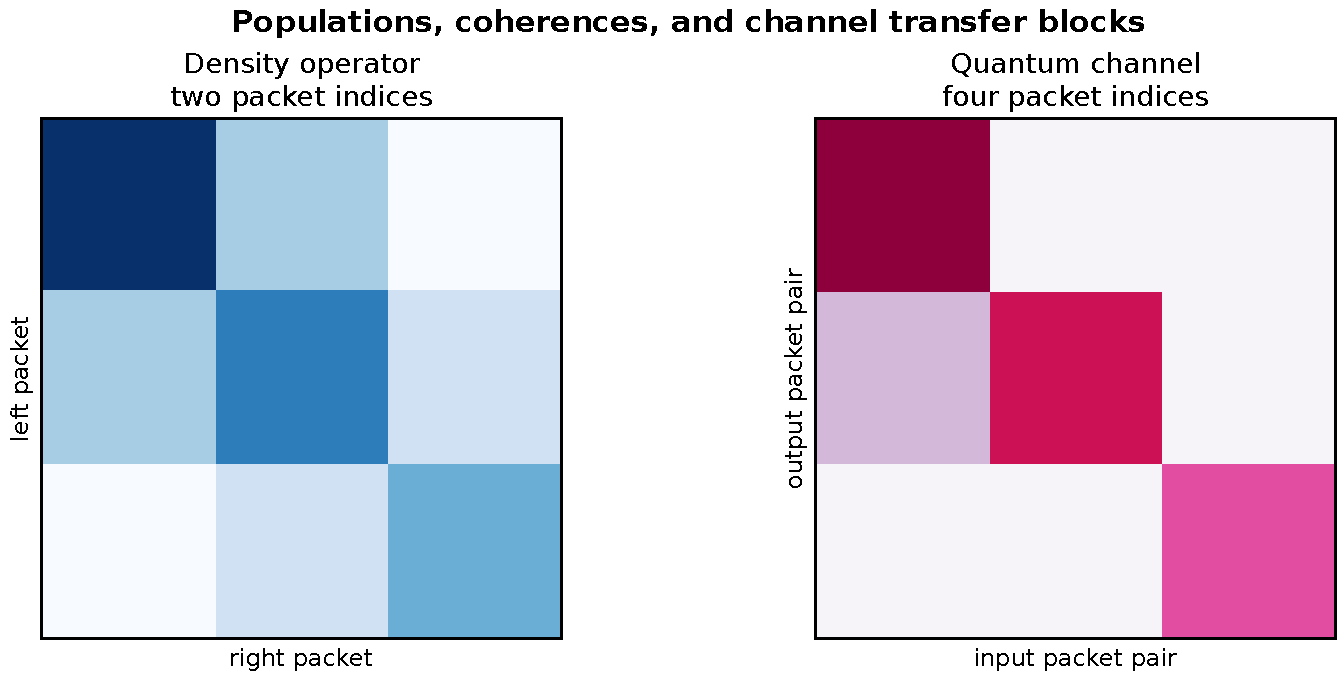
\includegraphics[width=.78\textwidth]{assets/s_channel_blocks.pdf}
\caption{State operators carry two packet indices, while channels act between pairs of packet labels.}
\end{figure}

\subsection{Polynomial operator-space collapse}
If only polynomially many density blocks are reachable and every block has a polynomial representation, then mixed-state evolution can also be simulated in polynomial time. The representation size is not the square of the full Hilbert dimension. It is the total cost of the active left-right blocks.

\begin{derivedbox}
For a polynomial active set $A_n$ of packet labels, a density-matrix simulator has at most $|A_n|^2$ label pairs. Polynomial-time simulation follows when each active coherence block has a polynomial classical representation and channel updates remain sparse and efficient.
\end{derivedbox}

\section{Channels, Kraus maps, and Lindblad generators}
\label{s:ch:channels}
\index{quantum channel}
\index{Lindblad equation}

\subsection{Four-index transfer}
A quantum channel with Kraus operators $K_\mu$ acts by
\[
\Phi(\rho)
=
\sum_\mu K_\mu\rho K_\mu^\dagger.
\]
Relative to operator packets
\[
\mathcal P_{\alpha\beta}(X)
=
P_\alpha X P_\beta,
\]
the channel has blocks
\[
\Phi_{\gamma\delta,\alpha\beta}
=
\mathcal P_{\gamma\delta}
\,\Phi\,
\mathcal P_{\alpha\beta}.
\]
Thus a channel carries four packet labels: an input coherence pair and an output coherence pair.

\subsection{Symmetry-preserving channels}
If every Kraus operator commutes with the symmetry action, the channel is diagonal in the isotypic labels. More generally, Kraus operators may carry definite charges, producing a sparse selection rule. Amplitude damping transfers population between number sectors. Dephasing damps selected off-diagonal blocks. Particle loss moves weight-$k$ population to weight $k-1$.

\subsection{Lindblad dynamics}
A Markovian open system obeys
\[
\frac{d\rho}{dt}
=
\mathcal L(\rho)
=
-i[H,\rho]
+
\sum_a
\left(
L_a\rho L_a^\dagger
-
\frac12\{L_a^\dagger L_a,\rho\}
\right).
\]
Packet selection rules of $H$ and $L_a$ determine a sparse directed graph on coherence pairs. If the reachable graph and each block representation remain polynomial, a classical integrator can evolve the reduced system.

\subsection{Error accounting for truncated channels}
Let $\Pi_A$ project operator space onto an active set of coherence blocks. A reduced evolution uses
\[
\mathcal L_A
=
\Pi_A\mathcal L\Pi_A.
\]
The discarded transfer is
\[
(I-\Pi_A)\mathcal L\Pi_A.
\]
Duhamel's formula yields an error bound analogous to the Hamiltonian leakage theorem. The resulting estimate depends on the induced norm of the discarded superoperator transfer and the integration time.

\subsection{Syndrome-conditioned recovery}
Error correction naturally fits the four-index model. Syndrome measurement selects a population packet, classical processing chooses a recovery, and the recovery transfers the state toward the code packet. A full simulation must still retain the logical state inside each syndrome sector.

\begin{frontierbox}
A useful open-system collapse theorem should state the norm, time horizon, packet-discovery algorithm, integration precision, and growth of reachable coherence pairs. Sparsity of a displayed block matrix is not enough by itself.
\end{frontierbox}

\section{Measurement, conditioning, and classical feedback}
\label{s:ch:measurement}
\index{measurement}

\subsection{Projective measurement}
For projectors $\{P_\alpha\}$, the probability of outcome $\alpha$ is
\[
p_\alpha
=
\Tr(P_\alpha\rho),
\]
and the conditioned state is
\[
\rho_\alpha
=
\frac{P_\alpha\rho P_\alpha}{p_\alpha}
\]
when $p_\alpha>0$. Measurement is therefore packet selection followed by normalization.

\subsection{Branching complexity}
A measurement-assisted circuit produces a tree of outcomes. Classical simulation is efficient when the branch distribution can be sampled or summed without enumerating exponentially many relevant histories. Symmetry can merge histories that lead to the same packet state, but only if the feedforward policy respects the same equivalence.

\subsection{Dynamic programming on packet states}
Suppose each branch is represented by a pair $(\alpha,r)$, where $\alpha$ is a packet label and $r$ is a compact internal state. If polynomially many distinct pairs occur at every depth, identical pairs can be merged and their probabilities added. This gives a dynamic program instead of an exponential branch tree.

\begin{proposition}[Branch-merging simulation]
Suppose a measurement-and-feedback circuit has polynomial depth and polynomially many distinct reachable packet representations at each step. Assume that the initial representation is efficiently constructible, each representation has a polynomial-time canonical key sufficient for all future transitions, all successor representations and their transition probabilities can be enumerated in polynomial time, and the final predicate is efficient. Then the final acceptance probability is classically computable to the requested polynomial precision in polynomial time. The same conclusion holds for any polynomially supported final output distribution.
\end{proposition}

\begin{proof}
Maintain a probability dictionary over distinct packet representations. Each measurement or controlled gate updates every entry into polynomially many successors. Merge equal successors. The dictionary remains polynomial by hypothesis.
\end{proof}

\subsection{Reset and dissipation}
Reset is nonunitary but often simplifies a classical representation by removing entropy or closing branches. Conversely, measurement may expose a classical label while leaving a complex logical state. The resource value of measurement depends on the target, ancilla convention, and cost function.

\subsection{Connection to catalytic gate models}
The larger gate-set monograph studies temporary excursions into measurement, ancilla, or symmetry-breaking resources. The present monograph asks a different question: when does the resulting model remain classically simulable? A temporary resource may shorten a quantum circuit without making the computation classically easy.

\section{Block encodings and polynomial operator transforms}
\label{s:ch:block-encodings}
\index{block encoding}

\subsection{Projector block form}
A block encoding places a generally nonunitary operator $A$ inside a larger unitary $U$ so that
\[
(\bra0\otimes I)
U
(\ket0\otimes I)
=
\frac{A}{\alpha}.
\]
With
\[
P_0=\ket0\bra0\otimes I,
\]
this is the selected block
\[
P_0UP_0
=
\frac{A}{\alpha}
\]
after identifying the encoded subspace.

\subsection{Structural connection}
The encoded operator is literally a projector block of a unitary. Polynomial transformations of singular values can be implemented by controlled phase sequences once the block encoding and access model are available. This makes block encodings a natural part of a projector calculus.

\subsection{Why block encoding does not imply classical simulation}
A block encoding can be efficient on a quantum computer because $U$ is supplied by an oracle or a succinct circuit. A classical algorithm may not have efficient access to the entries of $A$, to the block state, or to the polynomial transform. The selected block may still have exponential dimension.

\begin{scopebox}
The statement ``$A$ is a block of $U$'' is structural. A classical collapse requires a polynomial classical description of the active encoded state, efficient application of the selected block, and efficient evaluation of the output.
\end{scopebox}

\subsection{Symmetry-resolved block encodings}
If $A$ commutes with a symmetry group, both the encoded system and the ancilla can be decomposed into packets. A symmetry-resolved block encoding may reduce normalization, memory, or simulation cost for selected sectors. The relevant objects are
\[
P_\chi P_0 U P_0P_\psi.
\]
Exact symmetry removes off-diagonal $\chi\neq\psi$ blocks. Approximate symmetry yields leakage terms that must be included in the error budget.

\subsection{Research direction}
A useful classical theorem would identify access models in which the active block has polynomial packet dimension or a compact internal representation. This could cover structured sparse matrices, low-rank updates, association-scheme operators, and fixed-particle Hamiltonians.

\chapter{The complexity boundary}
\section{Compressed packet simulation}
\label{s:ch:compressed-packets}
\index{compressed representation}

\subsection{Beyond packet dimension}
The small-packet theorem stores one amplitude per packet-basis state. This is not the only classical representation. A state in an exponentially large packet may lie on a polynomially parameterized manifold. Stabilizer states, Gaussian states, matrix-product states of bounded bond dimension, and low-rank operator states are standard examples of compact internal encodings.

Let $\mathcal R_n$ be a class of classical descriptions, and let
\[
\operatorname{decode}:\mathcal R_n\to P_n\Hh_n
\]
associate a quantum state with each description.

\begin{theorem}[Compressed-packet simulation]
\label{s:thm:compressed-packet}
A polynomial-time uniform quantum circuit family lies in $P$ if there is a polynomial-size classical representation satisfying:

\begin{enumerate}
\item the initial state has an efficiently constructible description $r_0\in\mathcal R_n$;
\item every gate induces a polynomial-time update $r\mapsto T_j(r)$ with
\[
\operatorname{decode}(T_j(r))
=
G_j\operatorname{decode}(r);
\]
\item all intermediate description sizes remain polynomial;
\item the acceptance probability is computable from the final description in polynomial time.
\end{enumerate}
\end{theorem}

\begin{proof}
Iterate the polynomial-time classical updates on the polynomial-size descriptions and evaluate the final measurement. The algorithm never reconstructs the full state vector.
\end{proof}

\subsection{Two-axis complexity}
The records suggest the pair
\[
(D_{\rm packet},\chi_{\rm internal}),
\]
where $D_{\rm packet}$ measures active packet size or count and $\chi_{\rm internal}$ measures the representation cost inside the packet. Efficient simulation may follow from either coordinate:

\begin{itemize}
\item fixed weight has polynomial $D_{\rm packet}$ and can use explicit amplitudes;
\item stabilizer states may have exponential support but polynomial $\chi_{\rm internal}$;
\item Gaussian states may occupy large number sectors but have polynomial covariance descriptions;
\item half-filled generic states may have both coordinates exponential.
\end{itemize}

\begin{figure}[H]
\centering
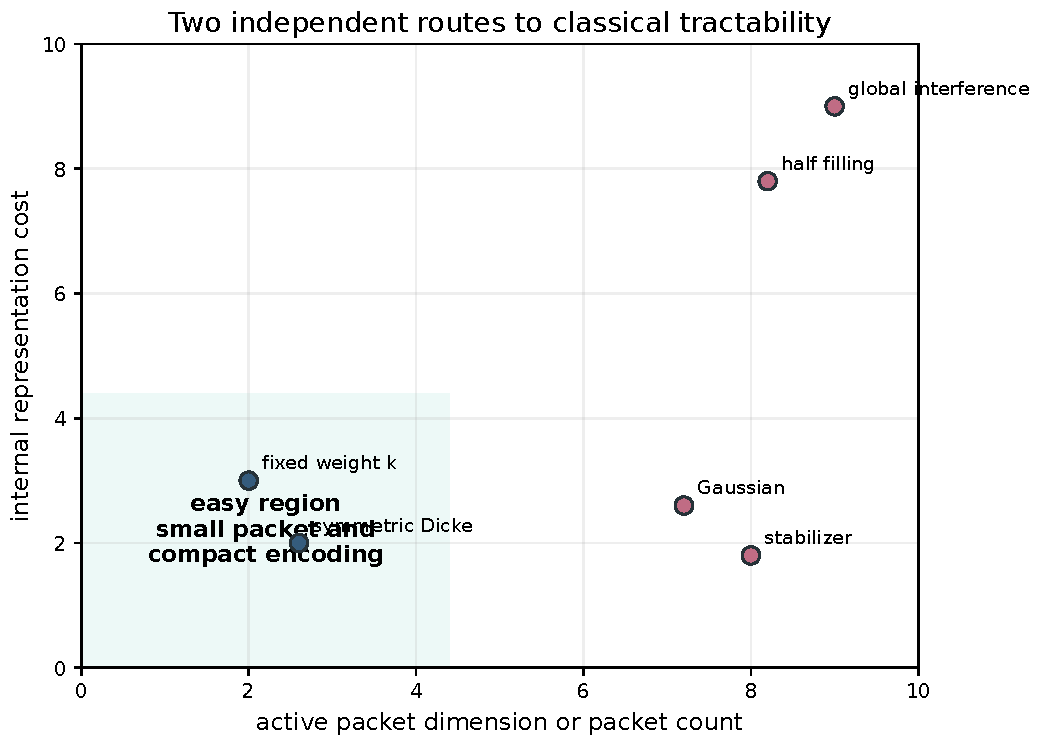
\includegraphics[width=.72\textwidth]{assets/s_two_axis_complexity.pdf}
\caption{Packet dimension and internal representation cost are independent classical resources.}
\end{figure}

\subsection{Hybrid transfer graphs}
Suppose packets are nodes of a sparse graph and each node carries an internal representation. A gate may update a node internally or transfer a compact component to neighboring nodes. The simulation cost depends on
\[
\sum_{\alpha\in A_t}\operatorname{size}(r_\alpha)
+
\#\{\text{nonzero transfers at time }t\}.
\]
This model combines symmetry selection rules with compact state classes.

\subsection{Closure is the decisive condition}
A compact representation may be destroyed by one gate. Clifford tableaux fail under generic non-Clifford rotations. Gaussian covariance matrices fail under generic non-Gaussian operations. Low-bond tensor networks may acquire exponential bond dimension. The theorem therefore requires closure or a proved polynomial growth bound, not merely a compact initial state.

\begin{principle}[Representation growth audit]
The correct complexity variable is the maximum representation size reached along the computation, not the size of the initial or final state alone.
\end{principle}

\section{Global interference and the failure of local packet collapse}
\label{s:ch:global-interference}
\index{Forrelation}
\index{interference}

\subsection{A different quantum mechanism}
Invariant-packet reduction succeeds when large parts of Hilbert space are never occupied or can be compressed locally. A different regime stores the answer in coherent relations among many paths. The individual amplitudes may be simple, while their signed sum is the computational object.

\subsection{Forrelation amplitude}
Let $f,g:\{0,1\}^n\to\{-1,1\}$ and $N=2^n$. The circuit with alternating Hadamards and phase oracles has zero-state amplitude
\begin{equation}
\Phi(f,g)
=
\frac1{N^{3/2}}
\sum_{x,y}
 f(x)(-1)^{x\cdot y}g(y).
\label{s:eq:forrelation}
\end{equation}
The circuit does not evaluate the $N^2$ terms separately. It preserves phases and lets them interfere.

\begin{figure}[H]
\centering
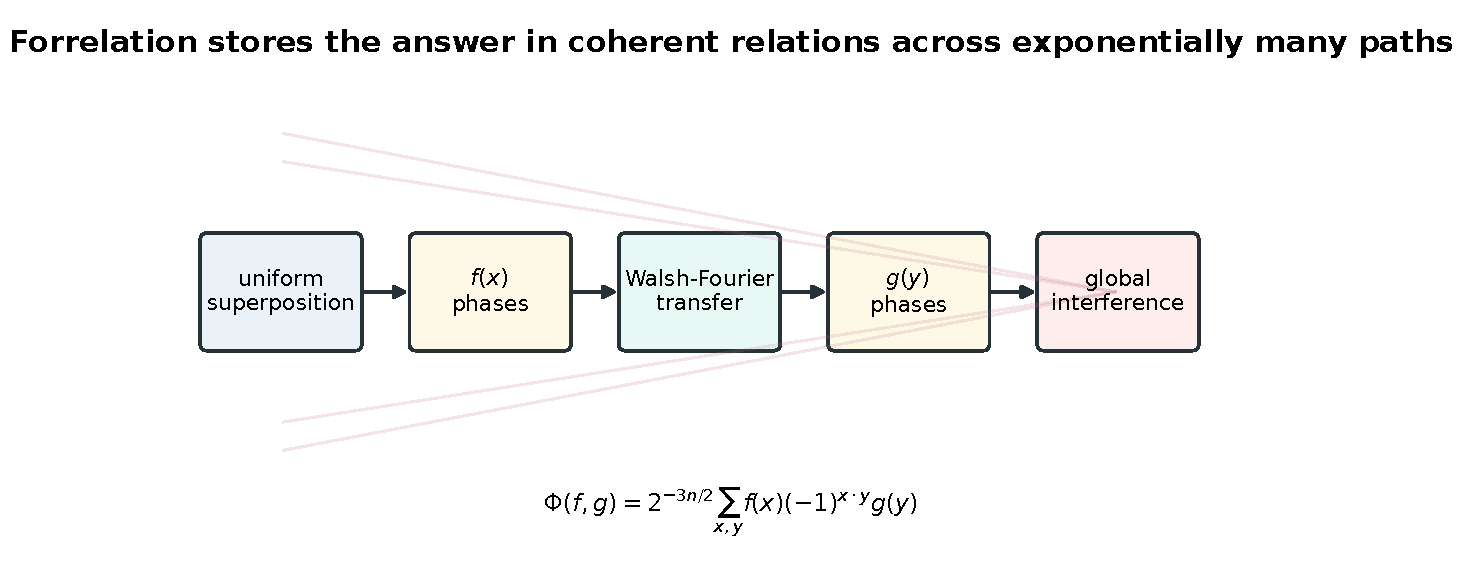
\includegraphics[width=.90\textwidth]{assets/s_forrelation_interference.pdf}
\caption{Forrelation is governed by coherent Fourier transfer rather than a small invariant sector.}
\end{figure}

\subsection{Why Fourier structure is not automatically easy}
The Walsh transform is explicit and highly symmetric. That does not imply that the bilinear expression in \cref{s:eq:forrelation} is classically polynomial-time computable when $f$ and $g$ are supplied through restricted query access. The difficulty lies in the access model and the coherent global relation, not in the absence of algebraic structure.

\subsection{Truth tables versus succinct access}
If the complete truth tables of $f$ and $g$ are part of the classical input, their length is already $N$, and an $O(N\log N)$ Walsh transform is polynomial in the explicit input length. In a query or succinct-circuit model, $n$ is the parameter and $N=2^n$. The same formula then represents exponentially many values.

This distinction illustrates a general rule: complexity statements must be measured against the input encoding. A quotient of exponential dimension may be efficient relative to an explicit matrix input but exponential relative to a succinct circuit input.

\subsection{Cross-packet coherence}
Suppose a projector family gives many packets $P_\alpha$. Even if each diagonal block is simple, the output can depend on the phases of
\[
P_\alpha\ket\psi
\quad\text{relative to}\quad
P_\beta\ket\psi
\]
for exponentially many pairs. A simulator that retains only populations
\[
\|P_\alpha\ket\psi\|^2
\]
loses this information. The hard-side invariant must measure classical compression of coherent relations, not merely active dimension.

\begin{frontierbox}
A representation-independent lower bound on interference compression for an explicit, succinct, uniform circuit family would be a major complexity result. The packet framework states the missing object but does not provide that lower bound.
\end{frontierbox}

\section{Simulation complexity versus decision complexity}
\label{s:ch:decision-complexity}

\subsection{Why simulator lower bounds are insufficient}
Showing that a circuit defeats one simulation strategy does not prove that its decision problem is outside $P$. A classical algorithm may compute the answer without reconstructing the quantum state. It is therefore insufficient to rule out only:

\begin{itemize}
\item full state-vector simulation,
\item one projector family,
\item bounded-width tensor-network contraction,
\item path sampling,
\item low-rank transfer matrices,
\item stabilizer decompositions,
\item any fixed catalogue of known simulators.
\end{itemize}

A proof of $P\neq BQP$ would need a lower bound against every deterministic polynomial-time classical algorithm for an explicit language.

\subsection{A representation-relative invariant}
For a declared classical representation class $\mathcal R$, define
\[
\operatorname{TC}^{\mathcal R}_\varepsilon(C)
=
\min\left\{
\operatorname{cost}(R):
R\in\mathcal R,
\ |R(C)-p_C|\le\varepsilon
\right\},
\]
where $p_C$ is the target acceptance probability. This permits a disciplined ladder:

\begin{enumerate}
\item exact polynomial-packet simulation for easy sectors;
\item lower bounds for local packet-query methods;
\item lower bounds for broader tensor, sampling, low-degree, and communication representations;
\item a representation-independent lower bound;
\item a separation of $P$ and $BQP$.
\end{enumerate}

Only the first step is completed here.

\subsection{Universal packetization and its consequence}
Consider the statement:

\begin{conjecture}[Universal polynomial packetization]
Every polynomial-time uniform quantum circuit family admits an efficiently discoverable exact or approximate packet representation of polynomial active size and polynomial transfer complexity, sufficient to compute its acceptance probability.
\end{conjecture}

If true, \cref{s:thm:poly-packet,s:thm:compressed-packet} would imply $BQP\subseteq P$, and hence $P=BQP$. The records do not establish this conjecture and explicitly identify global interference as an obstacle.

\subsection{The opposite route}
An explicit uniform family with a proved representation-independent classical lower bound and a polynomial quantum algorithm would establish $P\neq BQP$. The candidate succinct transfer-interference problem in the records illustrates the form of such a target, but the required lower bound is the unresolved theorem itself.

\begin{scopebox}
This monograph proves polynomial classical simulation for declared subclasses. It neither proves nor assumes a universal collapse of quantum computation.
\end{scopebox}

\subsection{Nonrelativizing issues}
Oracle separations show that query complexity can distinguish quantum and classical access. They also show why a black-box argument alone cannot settle ordinary $P$ versus $BQP$. A full separation would have to use explicit features such as uniform circuit generation, arithmetic structure, algebraic degree, communication constraints, or another nonrelativizing mechanism.

\section{Existence defects and quantum combinatorial realizations}
\label{s:ch:existence-defects}

\subsection{Metric collapse and existence collapse}
The simulation theorems compare costs of two realizations that both exist. A broader restricted-realization framework also allows the restricted object to be absent. If
\[
\mathcal R(x)=\varnothing,
\qquad
\mathcal A(x)\neq\varnothing,
\]
then enlarging the realization category changes feasibility rather than merely runtime.

\subsection{Quantum Latin-square example}
The order-six quantum-Latin-square record supplies an existence-level example. Entangled quantum Latin squares of order six exist, while mutually orthogonal non-entangled quantum Latin squares of order six do not. This is an ambient-versus-restricted realization gap, not a proof of classical simulation and not a gate-count shortcut.

The proof architecture uses support patterns, unitary-pattern constraints, graph orthonormal representations, projective-line closure, dimension contradictions, and a finite reduction to twelve classical Latin-square classes. Its conceptual relevance here is limited but useful: enlarging the allowed quantum resource can change whether a structure exists at all.

\subsection{Why this does not imply computational advantage}
Existence of an entangled combinatorial design does not by itself provide an algorithmic speedup. One must still specify an input problem, circuit family, output rule, and classical comparison. Likewise, nonexistence of a product realization does not prove classical hardness of the entangled realization.

\begin{scopebox}
The quantum Latin-square result is included as a contextual example of restricted-realization failure. It is not used as a premise in any packet-simulation theorem.
\end{scopebox}

\subsection{Unified terminology}
For a target $x$, let $c_{\rm res}(x)$ and $c_{\rm amb}(x)$ be minimum costs, with $+\infty$ assigned when a realization does not exist. Then
\[
\Delta(x)
=
c_{\rm res}(x)-c_{\rm amb}(x)
\]
includes both finite metric defects and infinite existence defects. Symmetry collapse concerns the special case where the ambient quantum description has a cheaper classical realization because its reachable representation is compressed.

\chapter{Algorithms and open directions}
\section{Architecture of a symmetry-collapse compiler}
\label{s:ch:compiler}
\index{compiler}

\subsection{The five-stage pipeline}
A practical compiler must perform more than symbolic block diagonalization.

\begin{enumerate}
\item Detect exact or approximate symmetries.
\item Construct an invariant basis, orbit quotient, or compact internal representation.
\item Compile each gate into that representation.
\item Track leakage, truncation, and numerical error.
\item Evaluate the requested measurement and emit a complexity certificate.
\end{enumerate}

\begin{figure}[H]
\centering
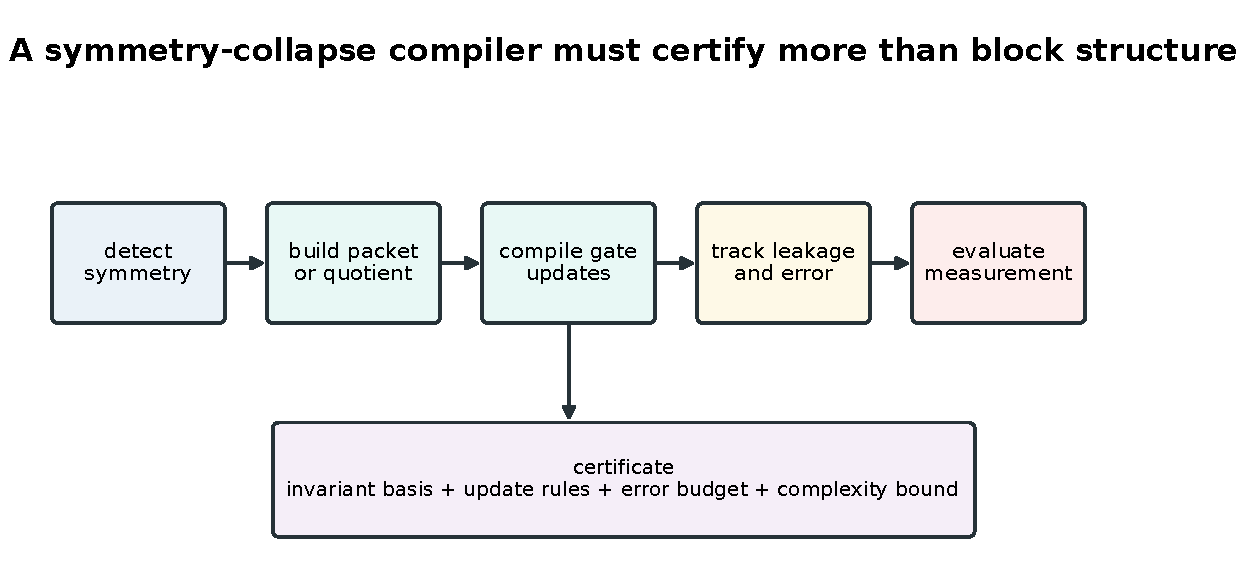
\includegraphics[width=.94\textwidth]{assets/s_compiler_pipeline.pdf}
\caption{A symmetry-collapse compiler and its required certificate.}
\end{figure}

\subsection{Symmetry detection}
Detection may use declared conserved quantities, commutators, finite-group generators, graph automorphisms, stabilizer relations, occupation conservation, or numerical approximate symmetries. Exact symbolic detection is preferable when available. Numerical detection must specify tolerances and how they propagate.

\subsection{Basis construction}
Examples include:

\begin{itemize}
\item subset indexing for fixed weight,
\item occupation vectors for bosons,
\item Dicke states for full permutation symmetry,
\item Schur coordinates for broader permutation symmetry,
\item orbit states for graph walks,
\item stabilizer tableaux,
\item fermionic or bosonic covariance matrices,
\item matrix-product states for bounded entanglement.
\end{itemize}

The compiler should avoid materializing an exponentially large change-of-basis matrix. It needs direct indexing and update formulas.

\subsection{Gate plan caching}
For a repeated circuit family, compile a packet plan containing affected index pairs, sparse matrix blocks, phase tables, and quotient couplings. The plan can be reused across parameter values when the sparsity pattern is fixed.

\subsection{Fallback and adaptive enlargement}
If a gate leaks from the current representation, the compiler can reject the reduction, merge packets, add neighboring sectors, or switch internal representations. The choice must preserve a certified error budget.

\subsection{Output certificate}
A useful machine-readable certificate should include:

\begin{itemize}
\item the symmetry or invariant-subspace proof,
\item active dimensions or representation sizes,
\item gate update complexity,
\item leakage or approximation bounds,
\item measurement complexity,
\item benchmark and hardware metadata,
\item the final complexity conclusion and its scope.
\end{itemize}

\section{Benchmark and validation protocol}
\label{s:ch:benchmark-protocol}

\subsection{Fair comparison}
A packet simulator and a full simulator should use the same precision, gate parameters, initial state, observable, and arithmetic path wherever possible. Report compilation separately from repeated application.

\subsection{Required metrics}
A complete benchmark should report:

\begin{enumerate}
\item full and reduced dimensions,
\item packet-discovery and compilation time,
\item one-shot runtime,
\item repeated-application runtime,
\item peak memory,
\item reconstruction or observable error,
\item symmetry leakage,
\item hardware and software versions,
\item number of repetitions over which compilation is amortized.
\end{enumerate}

\subsection{Algebraic and numerical validation paths}
For manageable $n$, embed a random packet state into the full space, apply identical gates in both representations, and compare final states. The included numerical validation program performs this check for structurally invariant fixed-weight circuits using complex floating-point arithmetic, with reconstruction tolerance $2\cdot10^{-12}$. The separate rational validation uses exact fractions and rational orthogonal gates. Exact subspace invariance is a property of the model, while near-machine-precision agreement is numerical evidence about this implementation.

\subsection{Scaling studies}
A scaling plot should include both fine packets and coarse packets. Fixed weight two demonstrates polynomial dimension. Parity demonstrates a constant-factor packet. Half filling demonstrates an exponential packet with a polynomial memory reduction factor. These controls prevent overinterpreting a speedup as a complexity collapse.

\subsection{Leakage tests}
Deliberately append a gate that breaks the proposed symmetry and verify that the simulator detects nonzero leakage. The archived tests break exact weight, parity, and weight modulo four, producing retained probabilities below one. A simulator that reports zero error after a symmetry-breaking gate without enlarging its representation is incorrect.

\subsection{Reproducibility contract}
The release preserves:

\begin{itemize}
\item the benchmark JSON data,
\item the Python figure generator,
\item packet and gate utilities,
\item exact rational checks and separately labeled numerical validation tests,
\item LaTeX source,
\item deterministic build commands,
\item checksums of final artifacts.
\end{itemize}

\begin{recordbox}
The release validation reproduces fixed-weight basis dimensions, residue partitions, symmetric/bosonic/fermionic dimension formulas, hypercube quotient symmetry, and full-vs-packet state reconstruction near machine precision.
\end{recordbox}

\section{Atlas of candidate symmetry collapses}
\label{s:ch:atlas}

\begin{figure}[H]
\centering
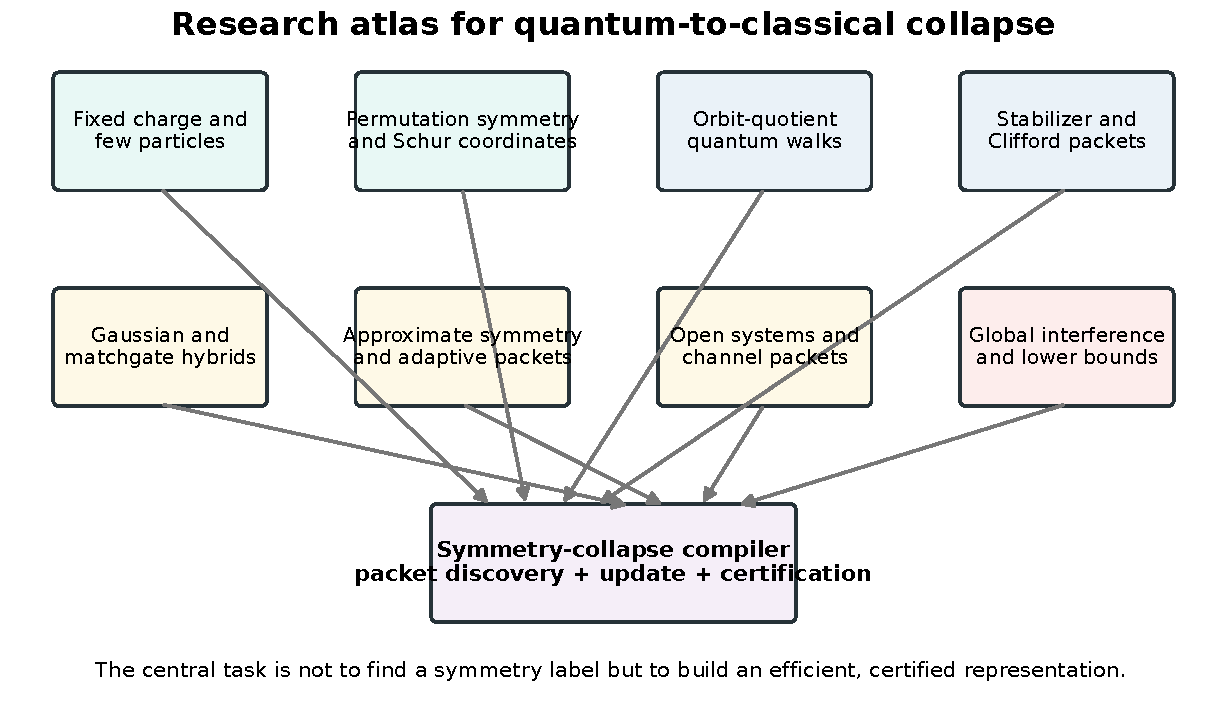
\includegraphics[width=.94\textwidth]{assets/s_research_atlas.pdf}
\caption{The main theorem and implementation directions organized around one certified compiler.}
\end{figure}

\subsection{High-confidence theorem families}
\begin{longtable}{@{}L{.25\textwidth}L{.33\textwidth}L{.32\textwidth}@{}}
\caption{High-priority collapse families.}\\
\toprule
Family & Compression mechanism & Decisive condition\\
\midrule
\endfirsthead
\toprule
Family & Compression mechanism & Decisive condition\\
\midrule
\endhead
Fixed charge $k=O(1)$ & Explicit subset basis of size $\binom nk$ & Number-preserving gates and efficient measurement\\
Permutation-symmetric qubits & Dicke basis of size $n+1$ & Collective or permutation-invariant dynamics\\
Symmetric qudits, fixed $d$ & Occupation basis $\binom{n+d-1}{d-1}$ & Efficient occupation-space updates\\
Polynomial-orbit walks & Quotient Hamiltonian on orbit states & Succinct quotient entries and orbit-invariant input/output\\
Few bosons or fermions & Fixed-particle occupation basis & Fixed particle number and efficient few-body updates\\
Stabilizer circuits & Tableau representation & Clifford closure and efficient Pauli measurement\\
Gaussian circuits & Covariance representation & Gaussian closure and efficient observable evaluation\\
\bottomrule
\end{longtable}

\subsection{Hybrid theorem targets}
The strongest new classes may combine several resources:

\begin{itemize}
\item charge packets plus Gaussian covariance,
\item permutation packets plus bounded-bond tensor networks,
\item stabilizer tableaux plus a small syndrome transfer graph,
\item orbit quotients plus Fourier diagonalization,
\item adaptive approximate packets plus rigorous leakage accounting.
\end{itemize}

\subsection{Negative controls}
A research atlas should preserve cases that do not collapse:

\begin{itemize}
\item parity alone,
\item weight modulo a fixed constant,
\item half filling with generic internal states,
\item a syndrome label with exponentially many logical qubits,
\item a block encoding without classical access,
\item global phase interference without a compact representation.
\end{itemize}

\subsection{Priority order}
The recommended sequence is:

{\small
\begin{enumerate}[nosep,leftmargin=*,label=\arabic*.]
\item implement the Dicke and orbit-quotient simulators;
\item combine fixed charge with Gaussian and stabilizer encodings;
\item develop adaptive leakage-certified packet growth;
\item build open-system four-index packet compilers;
\item search for broader representations of global interference;
\item separate simulator-specific lower bounds from decision-problem lower bounds.
\end{enumerate}
}

\section{Open problems}
\label{s:ch:open-problems}

\subsection{Efficient hidden-symmetry discovery}
\begin{question}
Which uniform circuit families have polynomial-dimensional invariant subspaces that can be discovered in polynomial time from the circuit description?
\end{question}
A nonconstructive invariant subspace does not yield an algorithm. The problem includes symbolic commutant computation, graph-orbit discovery, representation decomposition, and approximate invariant-subspace detection.


\subsection{Moving-frame discovery}
\begin{question}
Which circuit families admit efficiently computable frames \(W_t\) that expose one fixed polynomial packet even though no fixed laboratory-frame symmetry is preserved?
\end{question}
The theorem is exact, but the discovery problem is the substance. Useful frames must have compact descriptions and restricted gate matrices that can be generated without solving the original simulation problem.

\subsection{Permutation-commutant compilers}
\begin{question}
For which succinct permutation-invariant Hamiltonians and channels can all Schur-commutant block updates be generated in polynomial time without explicitly performing the full Schur transform?
\end{question}
The parameter count is polynomial for fixed local dimension. The remaining algorithmic issue is efficient block access.

\subsection{Dynamic packet graphs}
\begin{question}
Can local selection rules guarantee polynomial growth of the reachable packet graph for polynomially long circuits with weak but repeated symmetry breaking?
\end{question}
Bounded excitation gives one exact theorem. Broader results may require locality, energy penalties, or cancellation of packet-transfer paths.

\subsection{Minimal packet complexity}
\begin{question}
Given a circuit and error tolerance $\varepsilon$, what is the minimum active representation size among all efficiently applicable exact or approximate packet decompositions?
\end{question}
This optimization should include internal encoding and transfer sparsity, not only projector rank.

\subsection{Adaptive leakage}
\begin{question}
Can one prove polynomial active packet growth for physically local Hamiltonians with weak symmetry breaking over polynomial time?
\end{question}
The commutator bound is local in time and often conservative. Stronger bounds may use energy gaps, locality, Lieb--Robinson estimates, or destructive interference among leakage channels.

\subsection{Permutation and Schur compilers}
\begin{question}
Which noncollective but globally permutation-invariant circuit layers admit sparse Schur-basis updates without constructing the full Schur transform?
\end{question}

\subsection{Orbit quotients under succinct access}
\begin{question}
For which succinct graph families are orbit counts, orbit sizes, and quotient couplings computable in polynomial time without enumerating the graph?
\end{question}

\subsection{Hybrid Gaussian and packet methods}
\begin{question}
Can a polynomial number of non-Gaussian packet corrections be maintained on top of a Gaussian reference for broad interacting few-particle dynamics?
\end{question}

\subsection{Open systems}
\begin{question}
When does the number of reachable population and coherence blocks remain polynomial under a local Lindblad generator?
\end{question}

\subsection{Universal packetization}
\begin{question}
Is every polynomial-size quantum circuit classically compressible by some efficiently discoverable representation of polynomial size?
\end{question}
A positive answer would imply $P=BQP$. The record does not support this as a universal empirical principle.

\subsection{Interference lower bounds}
\begin{question}
Can one prove an explicit representation-independent exponential lower bound for the classical cost of the coherent interference needed by a uniform BQP language?
\end{question}
This is the hard-side frontier. Lower bounds against one simulator family are intermediate results, not the final theorem.

\begin{frontierbox}
The most achievable next theorem is not a universal complexity result. It is a complete compiler theorem for one new symmetry family, with explicit discovery, update, measurement, and leakage algorithms.
\end{frontierbox}

\section{Conclusion}
The quantum state vector is a universal coordinate system, not always the computationally intrinsic one. Conserved charges, finite-group representations, permutation orbits, few-particle sectors, and operator packets can expose much smaller dynamics. When the packet is efficiently discoverable, polynomial in size, closed under the gates, and compatible with the measurement, the quantum computation collapses exactly to a deterministic classical polynomial-time simulation.

The strongest current examples are concrete. Fixed charge at constant particle number is polynomial. Exact charge conservation is not necessary: moving packet schedules, efficiently computable moving frames, and bounded unions of low-excitation sectors also collapse to polynomial classical simulation. Fully symmetric fixed-local-dimension dynamics is polynomial. A stronger mixed-state theorem compresses all permutation-invariant Schur sectors into a polynomial commutant record, with $O(n^3)$ density-matrix parameters for qubits under efficient block access. Polynomial-orbit walks are polynomial under quotient-access hypotheses. Few-particle bosonic and fermionic systems are polynomial under efficient updates, while growing particle number gives a sharp progression through quasipolynomial, subexponential, and exponential sector sizes. Stabilizer and Gaussian representations show that an exponential packet can also be easy when its internal states admit compact closed coordinates. Recorded number-conserving benchmarks show large memory and repeated-application gains with zero reconstruction error at the recorded precision.

The boundaries are equally sharp. Parity, modulo-four charge, and half filling do not generally change exponential scaling. Entanglement can remain hard inside one packet. A syndrome label does not compress logical information. A block encoding does not provide a classical access model. Global Fourier interference may be fully structured yet resist small packetization. Symmetry collapse is therefore not a slogan that all quantum computation is classical. It is a theorem architecture for identifying substantial subclasses that are.

The core research invariant is the complete classical representation record
\[
\bigl(
\text{discovery cost},
N_{\rm packets},
D_{\rm internal},
S_{\rm transfer},
L_{\rm leakage},
\text{measurement cost}
\bigr).
\]
A future compiler that computes and certifies this record can decide when the full state vector is unnecessary, when a hybrid representation is preferable, and when symmetry alone is insufficient.

